\documentclass[useAMS,usenatbib]{mn2e}
%\documentclass[twocolumn]{emulateapj}
\usepackage{graphicx,natbib,color,multirow,amsmath,url,soul}
\usepackage{epsfig}
\usepackage{float}
\usepackage{deluxetable}
\newcommand{\s}{$_{\rm s}$}
\newcommand{\kms}{km~s$^{-1}$}
\newcommand{\msun}{{\it M}$_{\odot}$}
\newcommand{\lsun}{{\it L}$_{\odot}$}
\newcommand{\mear}{{\it M}$_{\oplus}$}
\newcommand{\etal}{{\it et al.}}
\newcommand{\ie}{{\it i.e.}}
\newcommand{\eg}{{\it e.g.}}
\newcommand{\be}{\begin{equation}}
\newcommand{\ee}{\end{equation}}
\newcommand{\magarc}{{\rm mag\,arcsec$^{-2}$}}
\newcommand{\MK}{{{\rm M}_{\rm ext,K}-5\log h}}
\newcommand{\ri}{{$r_{21}$}}
\newcommand{\ra}{$R_A$}
\newcommand{\vobs}{{v_{\rm obs}}}
\newcommand{\kmsMpc}{km~s$^{-1}$ Mpc$^{-1}$}
\newcommand{\h}{$h_{70}$}
\newcommand{\vpec}{v_{\rm pec}}
\newcommand{\like}{{\mathcal L}}
\newcommand{\vs}{\vspace*{5pt}}
\newcommand{\continued}{ (Continued)}
\newcommand{\radr}{\textsc{petroR90\_r}}


\newcommand{\ferengi}{\textsc{ferengi}}
\newcommand{\hst}{\textit{HST}}
\newcommand{\hubble}{\textit{Hubble Space Telescope}}
\newcommand{\subaru}{\textit{Subaru}}
\newcommand{\sextractor}{\textsc{SExtractor}}
\newcommand{\galapagos}{\textsc{Galapagos}}
\newcommand{\galfit}{\textsc{GALFIT}}
\newcommand{\gimtwod}{\textsc{GIM2D}}
\newcommand{\sersic}{S\'{e}rsic}






% Galaxy Zoo
\newcommand{\ffeatures}{$f_{\rm features}$}
\newcommand{\ffeaturesz}{$f_{\mathrm{features,}z}$}
\newcommand{\ffeaturesrest}{$f_{\mathrm{features,}z=0.3}$}
\newcommand{\ffeaturesdebiased}{$f_{\mathrm{features,debiased}}$}
\newcommand{\fbest}{$f_{\mathrm{features,best}}$}
\newcommand{\fodd}{$f_{\mathrm{odd}}$}
\newcommand{\fbar}{$f_{\mathrm{bar}}$}
\newcommand{\fclumpy}{$f_{\mathrm{clumpy}}$}
\newcommand{\fsmooth}{$f_{\rm smooth}$}
\newcommand{\fartifact}{$f_{\rm artifact}$}

\newcommand{\fHI}{f_{\rm HI}}
\newcommand{\zsim}{$z_{\mathrm{sim}}$}

% Bands

\newcommand{\Bband}{$B_{435W}$}
\newcommand{\Vband}{$V_{606W}$}
\newcommand{\iband}{$i_{775W}$}
\newcommand{\Iband}{$I_{814W}$}
\newcommand{\zband}{$z_{850LP}$}

% GZH subsamples

\newcommand{\main}{\texttt{main}}
\newcommand{\faded}{\texttt{faded}}
\newcommand{\recolored}{\texttt{recoloured}}
\newcommand{\goods}{\texttt{goods-shallow}}
\newcommand{\stripe}{\texttt{stripe-82-single}}
\newcommand{\coadd}{\texttt{stripe-82-coadd}}
\newcommand{\redshifted}{\texttt{redshifted}}
\newcommand{\simagn}{\texttt{simulated-agn}}




\newcommand\ion[2]{[#1$\;${\scshape{#2}}]}      % ion, i.e., [CII] = \ion{C}{ii}
\newcommand\pfeatures{$p_{\rm{features~or~disc}}$}
\newcommand\plusminus[2]{\genfrac{}{}{0pt}{}{#1}{#2}}
\newcommand\pnotedgeon{$p_{\rm{not~edge-on}}$}
\newcommand\pbar{$p_{\rm{bar}}$}
\newcommand\pnobar{$p_{\rm{no~bar}}$}
\newcommand\gztwo{Galaxy~Zoo~2}
\newcommand\mbh{$M_{\rm{BH}}$}
\newcommand\db{$d_{\rm{B-NB}}$}
\newcommand\fb{$f_{\rm{B>NB}}$}
\newcommand\pasa{PASA}
\voffset-1.25cm
\begin{document}

\title[Galaxy~Zoo~Hubble: passive red discs]{Galaxy~Zoo~Hubble: the evolution of red disc galaxies since $z=1$}
\author[Galloway et~al.]{\parbox[t]{16cm}{Melanie A. Galloway$^{1}$, Steven P. Bamford$^{3}$, Melanie Beck$^{1}$,
Hugh Dickinson$^{1}$ Lucy F. Fortson$^{1}$, Chris J. Lintott$^{4}$, Karen L. Masters$^{5,6}$, John I. Phillips$^{1}$, Claudia Scarlata$^{1}$,
B.D. Simmons$^{4,7}$\footnote{Einstein Fellow}, Kyle W. Willett$^{1}$
\vspace{0.1in} }\\
$^{1}$School of Physics and Astronomy, University of Minnesota, 116 Church St. SE, Minneapolis, MN 55455, USA \\
$^{2}$Department of Physics and Astronomy, University of Kentucky, 505 Rose St., Lexington, KY 40506, USA \\
$^{3}$School of Physics and Astronomy, The University of Nottingham, University Park, Nottingham, NG7 2RD, UK \\
$^{4}$Oxford Astrophysics, University of Oxford, Denys Wilkinson Building, Keble Road, Oxford, OX1 3RH, UK \\
$^{5}$Institute for Cosmology and Gravitation, University of Portsmouth, Dennis Sciama Building, Burnaby Road, Portsmouth, PO1 3FX, UK \\
$^{6}$SEPnet, South East Physics Network, UK \\
$^{7}$Center for Astrophysics and Space Sciences, Department of Physics, University of California, San Diego, CA 92093, USA \\
   }
\maketitle

\begin{abstract}
We study the evolution of the passive disc population from $z=1$ to $z=0.3$ in a sample of 20,000 galaxies from the COSMOS field and morphologically classified by the Galaxy Zoo: Hubble project. We find the fraction of discs occupying the red sequence, as well as the fraction of disc galaxies that are red, to decrease for the most massive galaxies ($\rm log(M/M_{\odot})>11$) but increase for lower masses. Our observations are consistent with a physical scenario in which more massive galaxies are more likely to enter a red disc phase, and more massive red discs are more likely to morphologically transform into ellipticals than their less massive counterparts. This paper also introduces a new method for using artificially-redshifted galaxies to quantify the redshift-bias in Galaxy Zoo classifications in order to accurately measure the fraction of disc galaxies as a function of redshift.  


\end{abstract}

\section{Introduction}
\label{sec:Intro}

Passive, red discs are an unconventional class of galaxies. They do not adhere to the standard bimodality of the colour-morphology relationship, whereby most galaxies tend to exist in one of two populations: blue, late-type discs exhibiting active star formation, and red, early-type ellipticals showing little to no signs of recent star formation \citep{Strateva2001, Baldry2004, Correa2017}. The division between the two populations is particularly apparent when represented visually on a colour-magnitude or colour colour diagram. Galaxies tend to populate in two distinct regions: the ``red sequence'' in the upper band, which contains predominantly early-type galaxies, and the ``blue cloud'' in the lower, containing mostly late-type spirals. This relationship has been shown to hold for $\sim >$ 85\% of galaxies out to z $\sim$ 1 \citep{Bell2004,Cirasuolo2007,Mignoli2009} and possibly beyond \citep{Giallongo2005, vanDokkum2006, Franzetti2007, Cassata2008}. 

The relatively tight correlation between galaxy colour (which traces the stellar content) and morphology (which traces dynamical history) suggests an evolutionary link between the two. In the simplest interpretation, it could be deduced that galaxies tend to begin their lives as young, star-forming discs, until some mechanism (secular or external) causes star-formation to cease while the galaxy simultaneously undergoes a morphological transformation from disc to spheroidal. The growing evidence for a significant population of galaxies which breaks this relationship, however, insists on more nuanced interpretations of this model. 

The passive disc population has been a matter of interest for understanding the mechanisms driving the evolutionary link between colour and morphology since their initial discovery.  In one of the earliest documented reports of this class, \citet{VandenBergh1976} identified a set of spirals in the Virgo cluster which were forming stars ``much less vigorously'' than the other galaxies of the same type, which were dubbed ``anemic spirals''. Analysis of this population suggested the possibility of ``gentle'' quenching mechanisms which could shut off star-formation without disrupting the morphology (in contrast to violent processes such as mergers, which are capable of destroying the disc \citep{Bell2004,Negroponte1983,DeLucia2006,Springel2005}). The low gas content in the anemic spirals suggested that subtle environmental factors played a role in stripping the gas required to continue star-formation, a process commonly known now as ram-pressure stripping \citep{Gunn1972,Steinhauser2016}. 

Other studies have since investigated other possible mechanisms could lead to the formation of passive discs, and how significant of a contribution this population makes to understanding the full picture of galaxy evolution. Environment is believed to play a strong role in their formation; many studies for instance find passive spirals preferentially in high-density environments \citep{Dressler1999, Poggianti1999, Goto2003, Deng2009, Hughes2009}. \citet{Moran2006} model the star-formation histories of passive spirals at $z\sim0.4$ and find them to be consistent with models for spirals affected by gas-starvation \citep{Larson1980, Quilis2000, Bekki2002}. Environment plays a significant factor in this scenario, whereby the interaction of the galaxy with the intra-cluster medium halts the accretion of gas onto the galaxy, inhibiting star-formation and causing a quench without disrupting the morphology significantly. Their results did not argue that starvation was the only mechanism responsible for building up the population of discs in the red sequence, but do conclude that passive discs are indeed an important transition population.

\citet{Masters2010} is one of the few studies which finds no strong correlation of passive discs with environment, but do not rule out environment playing a significant contribution in their creation. They also find strong evidence for quenching via completely secular processes, given by their sample of passive discs being more massive and having a higher bar fraction than their star-forming counterparts. Massive galaxies are more likely to have been assembling for very long times, allowing sufficient time to use up all of their gas, without environment being a direct factor. This option could explain the observed correlations with density and passivity, given that higher-density regions were more likely to have been assembled at earlier times. Secondly, \citet{Masters2010} observed a significantly higher bar fraction in passive spirals (67\%) than star-forming spirals (27\%). Bars are known for their ability to efficiently drive gas to the centers of galaxies via a redistribution of angular momentum throughout the disc \citep{Sellwood1993,Shlosman1989,Ann2005}, which could increase central star-formation \citep{Hawarden1986,Ho1997} or feed the central supermassive black hole \citep{Athanassoula1992,Friedli1993}. The excess of bars in passive discs then suggests that bars were responsible for quickly using up the gas in the galaxy, resulting in subsequent quenching. 

Passive discs have thus far been proposed as both a final stage of galactic evolution, driven by secular and external processes capable of exhausting gas required for star-formation, and as a transition phase of galaxies toward a final evolution to red spheroidal, driven by processes which quench and morphologically transform on different timescales, or multiple separate processes acting independently. Understanding the significance of the passive disc population is therefore unquestionably an important key to understanding galaxy evolution as a whole. \citet{Bundy2010} investigates this subject by measuring the different morphological contributions to the red sequence since $z=1$, and estimate as high as 60\% of all galaxies go through a passive disc phase. It was not quantified which of these further evolve to spheroidal and which stay discs for the remainder of their lifetimes, but the decaying contribution of passive discs to $z=0.3$ was evidence that some fraction of these did indeed transform to elliptical.

This paper will investigate the evolution of the passive disc population from $z=1$ to $z=0.3$ using galaxies identified in the COSMOS field with morphological classifications from Galaxy Zoo: Hubble. We will measure the fraction of discs which are passive and the fraction of the red sequence occupied by discs as functions of mass and redshift, as well as the fractional contribution of red discs, blue discs, red ellipticals, and blue ellipticals to the total population. We will assess the mass-dependence of the significance of the red disc population, and discuss the likelihoods of the red disc phase being a transitory stage or an end-point of a typical galaxy's evolutionary path.

Section~\ref{sec:Data} will describe our methods for selecting disc galaxies and separating the sample into active / passive populations using a colour-colour diagnostic. In Section~\ref{sec:correction} we describe a new method of correcting for redshift bias in the detection of disc galaxies with Galaxy Zoo classifications using an artificially-redshifted set of images. In Section~\ref{sec:results} we present our results of the fraction of disc galaxies which are red, and the fraction of red sequence galaxies that are discs, as functions of mass and redshift. We compare our findings with results from the literature and discuss their implications in Section~\ref{sec:discussion}. Our main conclusions are outlined in Section~\ref{sec:conclusions}. We adopt a $\Lambda$CDM cosmology throughout this paper of $\Omega_m=0.31$ and $H_0=68~\rm km~s^{-1} Mpc^{-1}$ \citep{PlanckCollaboration2015}.


\section{Data}
\label{sec:Data}

The parent sample of galaxies in this paper is drawn from the Galaxy Zoo: Hubble (GZH) catalog \citep{Willett2016}, which provides morphological classifications for galaxies sourced from the HST Legacy Surveys. From the main catalog we select galaxies with imaging from the Cosmic Evolution Survey (COSMOS, \citet{Scoville2007}) in the redshift range $0.2<z<1$.  Rest frame NUV-r and r-J colours are taken from the UltraVISTA catalog \citep{McCracken2012,Ilbert2013}.

\subsection{Sample Selection}
\label{sec:sampleselection}

\begin{figure}
\centering
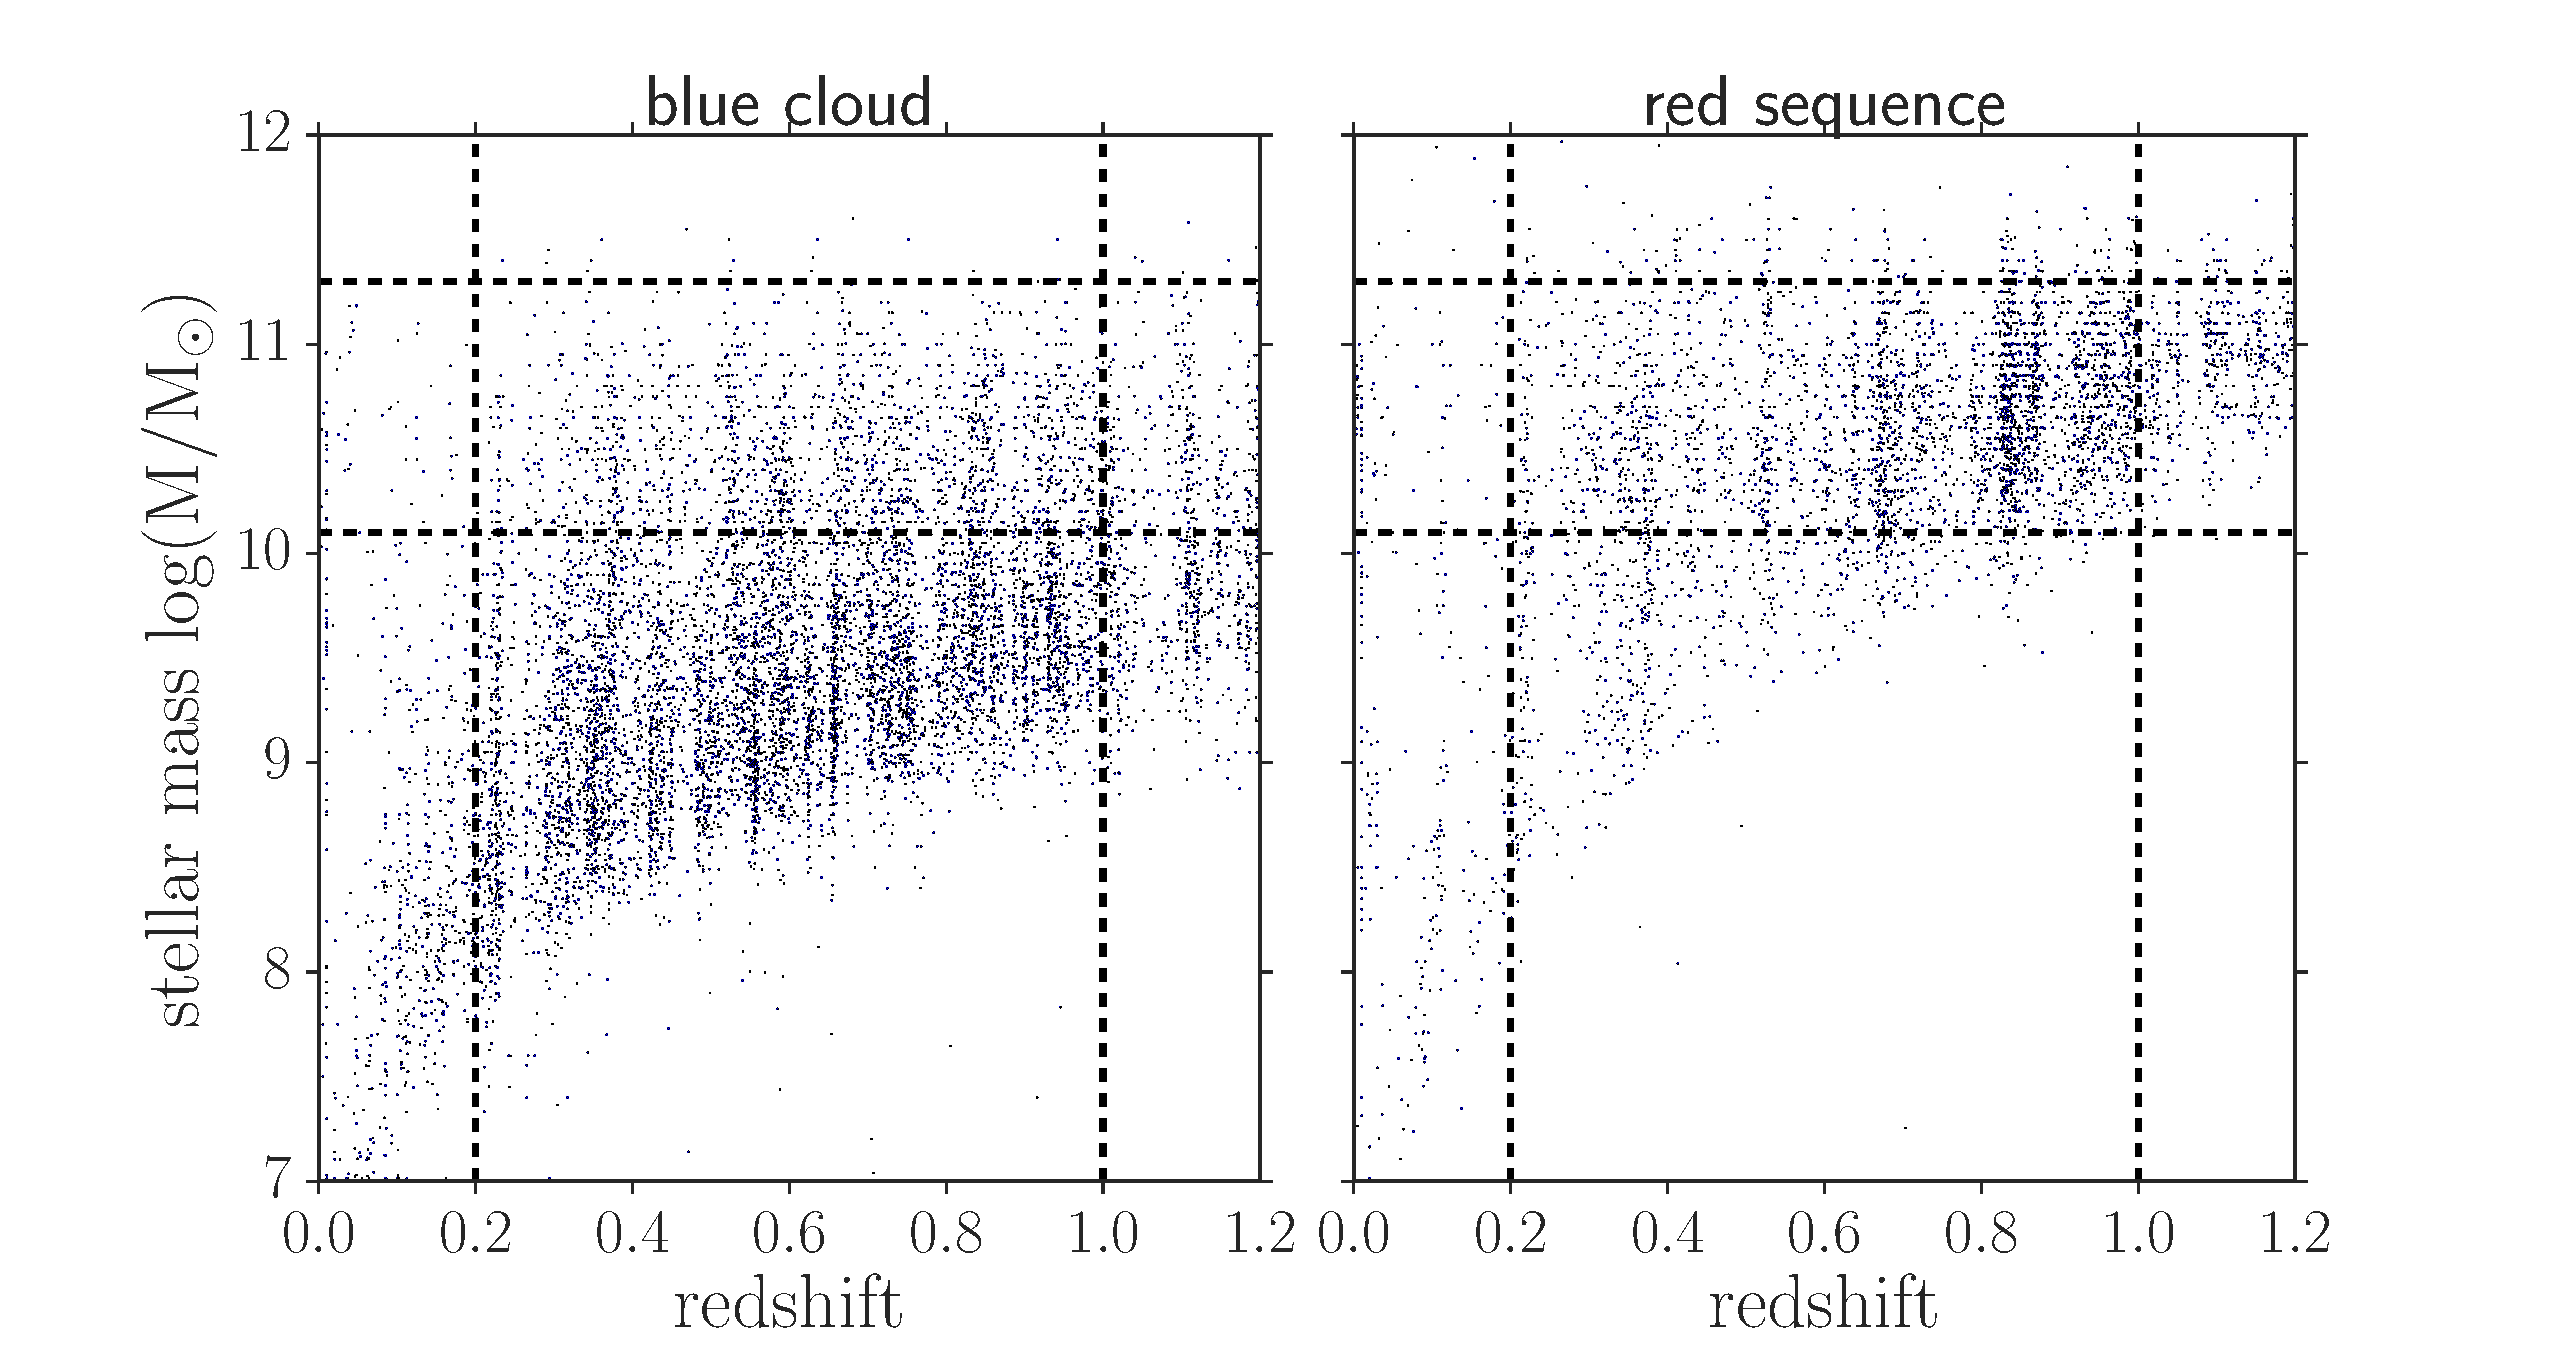
\includegraphics[width=0.5\textwidth]{figures/mass_selection.pdf}
\caption{[apologies this is not an aesthetically pleasing plot yet... comments on making it so are welcome.] The box enclosed by the dotted lines displays our mass-limited sample, defined as $0.2<z<1$ and $10.15<log(M/M_{\odot})<11.15$. Red sequence and blue cloud galaxies are plotted separately to illustrate the difference in limiting magnitudes for galaxies whose fluxes are dominated by I-band vs. V-band light respectively. It can be seen here that the mass cut of at least $log(M/M_{\odot})>10.15$ is effective for ensuring detection of all red galaxies out to $z=1$. Only random subset of points are displayed for clarity.}
\label{masscut}
\end{figure}

We identify a mass-limited sample of 20,811 disc and elliptical galaxies using the morphological classifications provided by GZH. Figure~\ref{masscut} shows the mass/redshift distribution of the parent blue cloud and red sequence galaxies, where the dashed lines indicate the limits $0.2<z<1.0$ and $10.15<log(M/M_{\odot})<11.15$ used for this study. Mergers and irregulars are excluded from the analysis by applying cuts of $\rm f_{irregular} > 0.3$ and $\rm f_{merger} > 0.5$ for galaxies which have at least 20 ``yes'' votes for the question, ``Is there anything odd?''. Last, we apply an inclination limit using $f_{\rm not~edge-on} > 0.3$ and $N_{\rm not~edge-on}>10$. Before applying this cut, it was observed that the red sequence region of the sample was dominated by highly-inclined galaxies, shown in Figure~\ref{fig:edgeon}. Given that galaxy colour should be independent of the angle in which it is observed, it is clear that the inclined galaxy colours are strongly affected by dust-reddening. While we are not using dust-corrected colours in our colour-colour separation, inclination has shown to have an affect on colours even in those which dust-corrected has been attempted \citep{Morselli2016a,Devour2017}. By limiting the sample to face-on galaxies, this bias should be removed (right panel of Figure~\ref{fig:edgeon}). 
 
\begin{figure}
\centering
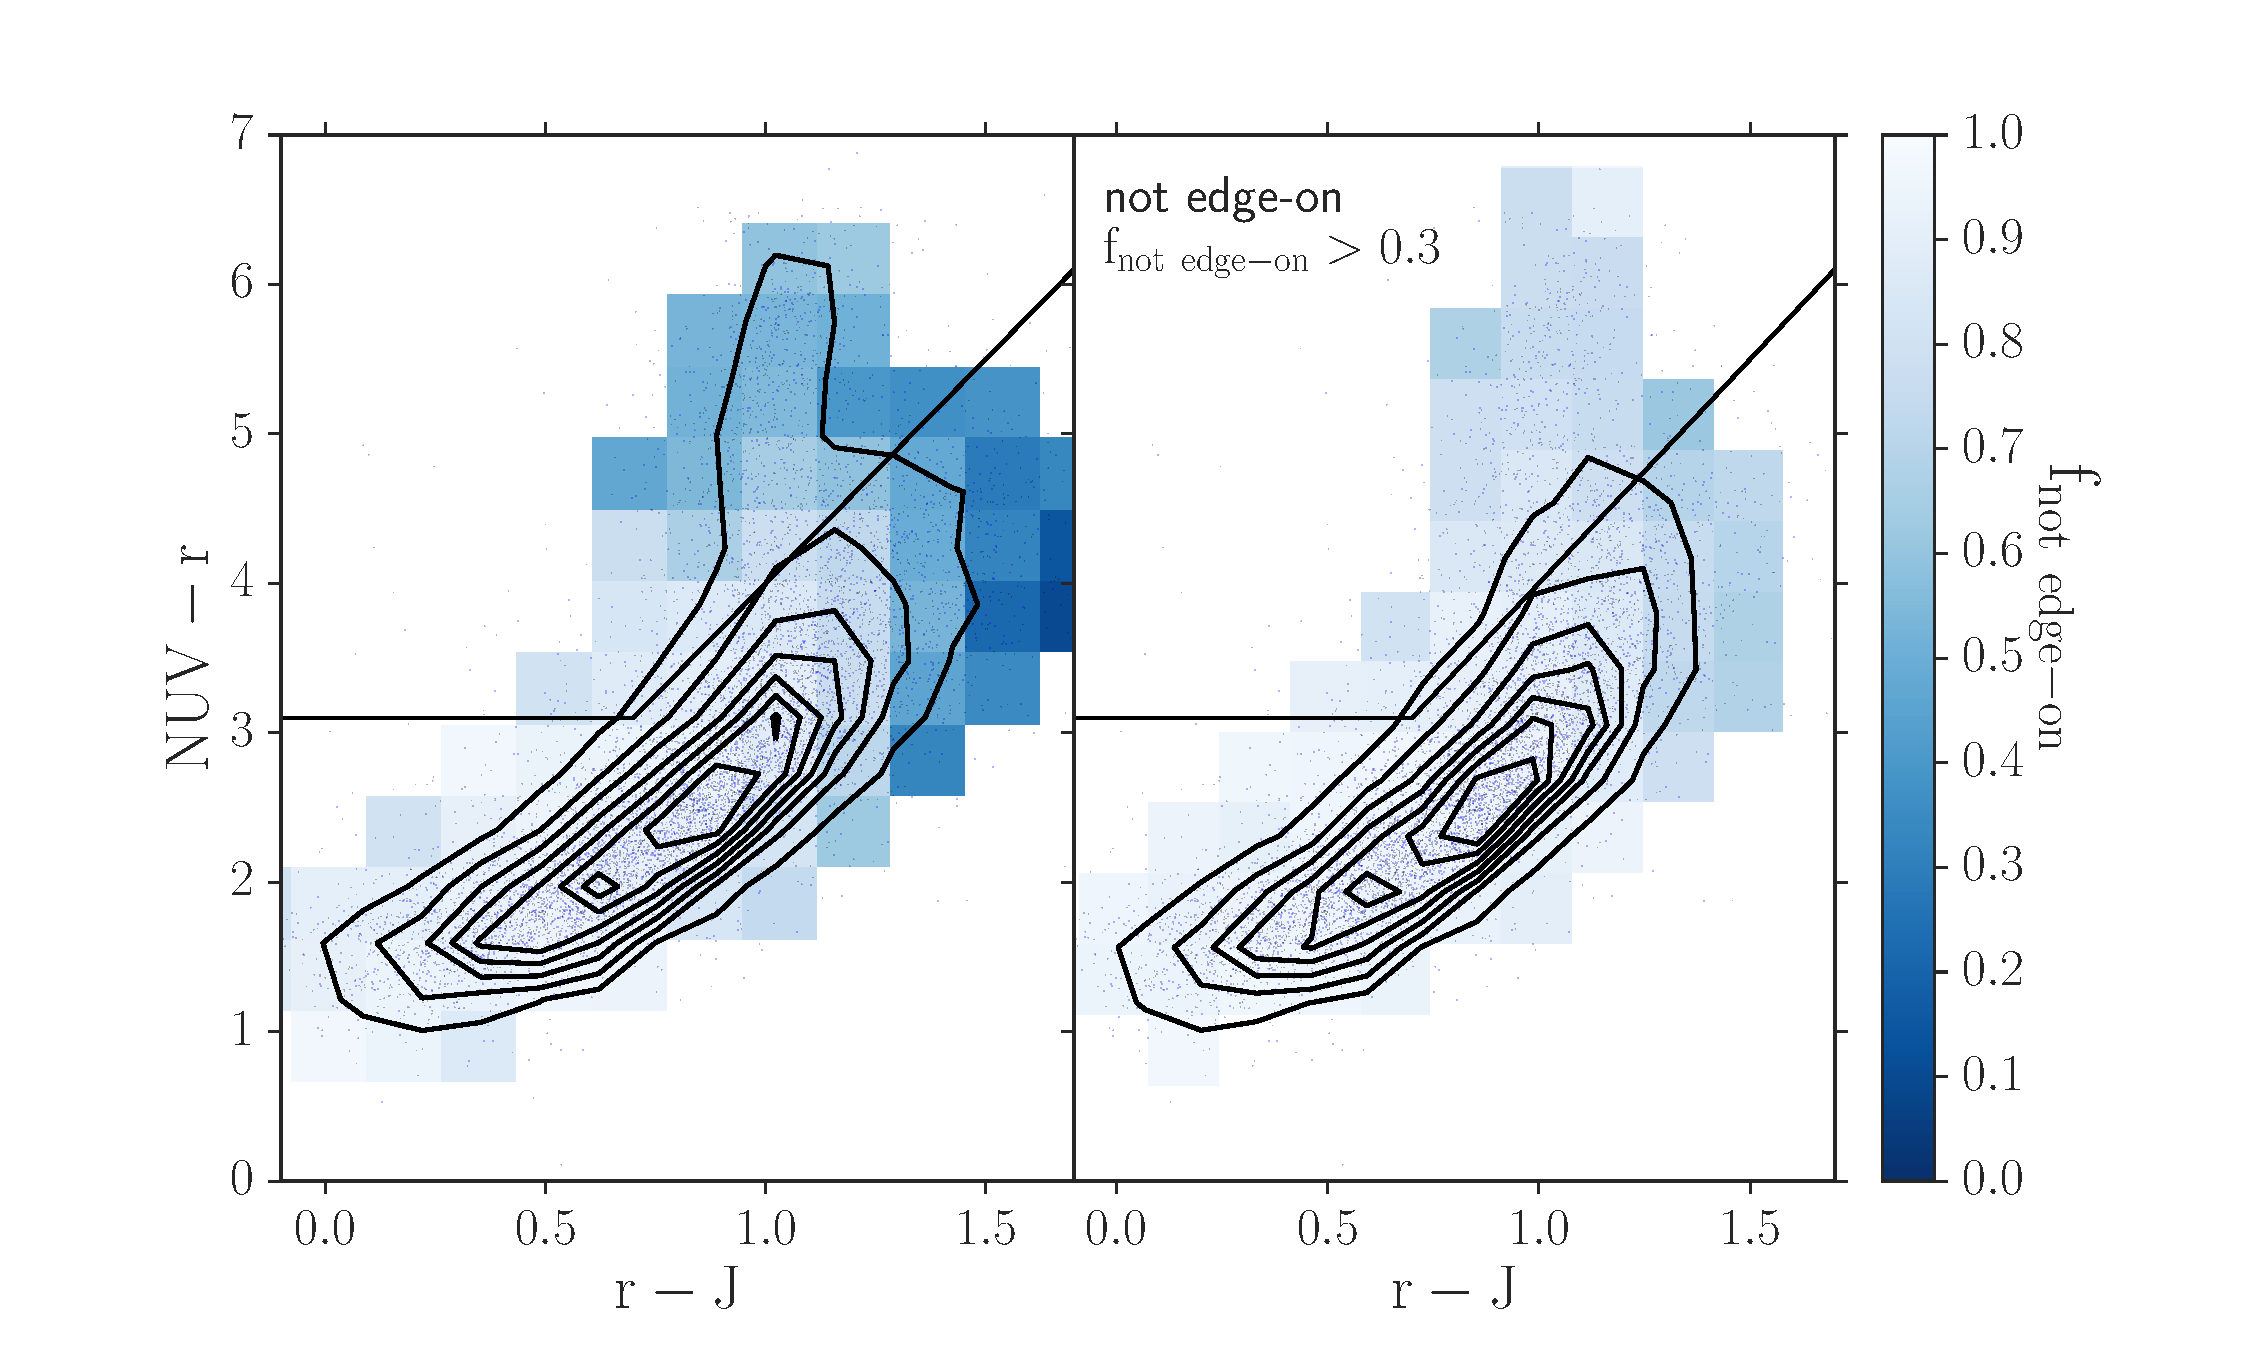
\includegraphics[width=3.5in,trim={1cm 0cm 1cm 1cm},clip]{figures/edgeon_colorcolor.pdf}
\caption{The effect of reddening for highly inclined galaxies. On the left panel is the distribution of $\rm f_{edge-on,no}$, which is the fraction of Galaxy Zoo users who voted ``no'' in response to the question ``Could this be a galaxy viewed edge-on?''. This vote correlates with inclination angle, such that low values represent highly inclined galaxies, and high values represent face-on galaxies. The bins are colored such that darker blue bins have a higher fraction of highly inclined galaxies, and white bins have high fractions of face-on galaxies. There is an obvious bias towards redder colours for galaxies with high inclination angles (low votes for $\rm f_{edge-on,no}$). We therefore implement a cut of $\rm f_{edge-on,no}>0.3$ to ensure that observed red colours are an indicator of a lack of star-formation, and not dust-reddening. }
\label{fig:edgeon}
\end{figure}
To classify the galaxies as quiescent or star-forming, a method similar to that described by \citet{Ilbert2013} (hereafter I13) was used, which implements a rest-frame NUV-$r$ versus $r$-J diagnostic. Here are some reasons these colours are great (NUV-r:) \citep{Arnouts2007a,Salim2005a,Wyder2007},\citep{Martin2007}

The demarcation line to separate the quiescent and active populations at $z=1$ is adopted from I13, which defines the quiescent galaxies as those which satisfy: $M_{NUV}-M_{r} > 3(M_{r}-M_{J})+1$ and $M_{NUV}-M_{r} > 3.1$. I13 applies this criteria to all galaxies in a range of $0.2<z<3$, although it performs best at separating the two populations in the redshift bin $0.7<z<1.2$, where $>98\%$ of galaxies identified as quiescent exhibited star formation rates less than $log(SFR) = -11$ (see Figure 3 of I13). Therefore this work uses the I13 separation criteria at $z=1$, and computes the evolution of the demarcation lines as a function of redshift to $z=0$. 

The evolution of $r-J$ and $NUV-r$ colours was measured using a stellar population synthesis model from \citet{Bruzual2003}. An instantanious-burst model (ssp) was chosen from the Padova1994 track to represent the colour evolution of a passively evolving galaxy, with a metallicity $Z=0.008=.4Z_{\sun}$, which is the typical metallicity of passive galaxies with mass $9 < log(M_{*}/M_{\odot}) < 10$ (\citet{Peng2015}, Figure 2a), chosen to correspond to the median mass of the sample ($log(M_{*}/M_{\odot})=9.7)$. A linear fit was geenerated for each colour within the range $0<z<2$, and the slopes for each were used to redefine the demarcation lines in five redshift bins: one with central value $z=0.007$ (used to classify the SDSS ferengi2 sample), and four with central values $z$ = [0.30,0.50,0.70,0.90] with widths $\Delta z=0.2$. The quiescent galaxies are thus defined in these bins as those that satisfy:

\begin{equation}
M_{NUV}-M_{r} > 3.1 + a_{1}(z)
\end{equation}

\begin{equation}
M_{NUV}-M_{r} > 3(M_{r}-M_{J} + a_{2}(z))+ a_{1}(z) + 1  
\end{equation}

where $a_{1}(z) = [0.54,0.38,0.27,0.16,0.05]$ and $a_{2}(z) = [0.19,0.14,0.10,0.06,0.02]$. 
% Figure - mag vs. z (needed??? questionable. useful? also questionable. ) 
%\begin{figure}
%\centering
%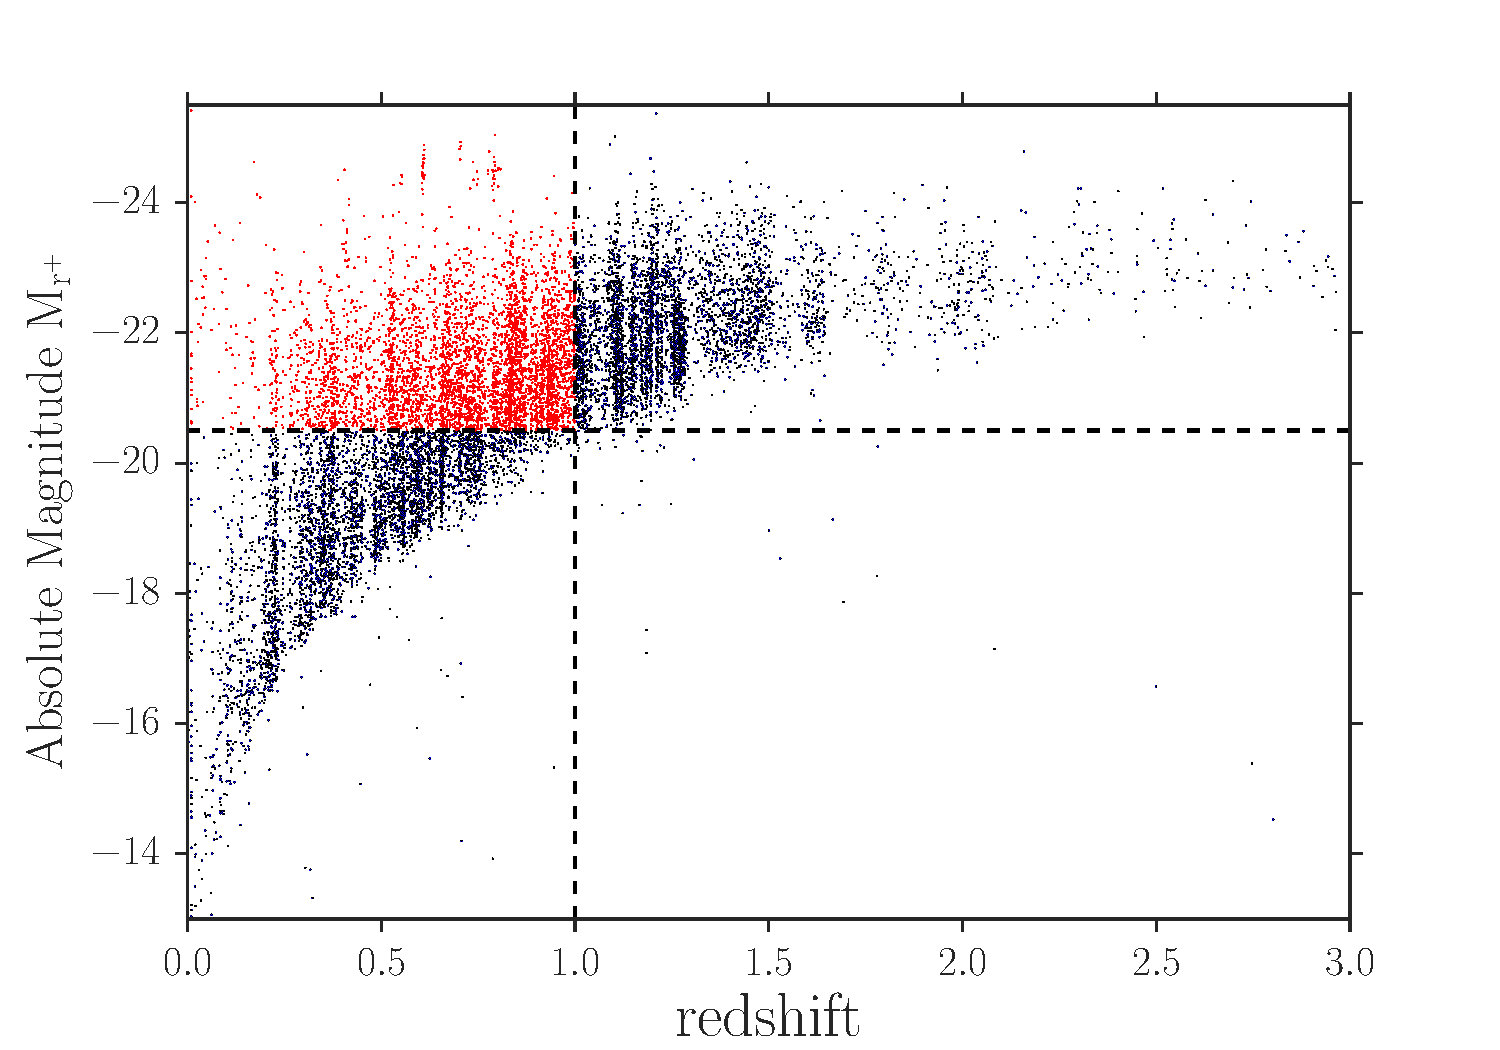
\includegraphics[width=3in]{figures/mag_z_limit.pdf}
%\caption{70,198 COSMOS galaxies cross-matched in GZH and UltraVISTA (all points). 27,584 are in volume-limited sample (red points).}
%\label{fig:volume_lim}
%\end{figure}   

We note that the evolution of the demarcation lines from $z=1$ to $z\sim0$ is very minimal, and our final results do not change if we perform the separation using static lines.


In describing our methods for separating active and passive populations using a colour-colour separation technique, we have used terminology such that blue/red have been used to describe colours explicitly, while active/passive have been used to describe ongoing/quenched star-formation. The remainder of this paper will assume that the colour cuts described in this section adequately separated the active and passive populations, and for convenience the terms red/blue will be used interchangeably with passive/active.  

\section{Correcting for Incompleteness in Disk Detection}
\label{sec:correction}
In this work, we study the growth of the red sequence population by evaluating the fraction of passive discs as a function of redshift, $\rm N_{red~discs}/(N_{red~discs}+N_{blue~discs})$, as well as the fraction of discs occupying the red sequence, $\rm N_{red~discs}/(N_{red~discs}+N_{red~ellipticals})$. To accurately measure these fractions, the number of discs and ellipticals populating each redshift interval must be known with confidence. To identify disc galaxies in our sample, we set a cut of $f_{\rm features}\ge0.3$, such that galaxies meeting this criteria are considered to have distinguishable features or disc structure (additional cuts are also placed to eliminate clumpy, highly inclined, and merging galaxies; see Section~\ref{sec:sampleselection}), and galaxies which do not are considered elliptical. However, it is known that distinguishing disc structure from spheroidal becomes increasingly challenging at high redshifts (for both experts and novice classifiers alike), where features are less resolved and more difficult to identify. \citet{Willett2016} show using a set of artificially-redshifted simulated galaxy images classified in Galaxy Zoo that vote fractions for the same galaxy can be drastically different measured at $z=1$ from $z=0$, often enough to change its morphological classification (we will show the same in Section~\ref{ssec:ferengi}).  Therefore it is predicted that applying a $f_{\rm features}$ cut to identify discs will increasingly underestimate their true number at increasing redshift intervals. A set of artificially redshifted images was used to quantify and correct for this incompleteness in disc and elliptical detection, described in the next section.
 
\subsection{FERENGI2 set of artificially redshifted galaxy images}
\label{ssec:ferengi}
\ferengi2 is a set of simulated galaxy images created using the \ferengi{} code \citep{Barden2008}. These were created from a parent sample of 936 nearby ($z<0.01$) SDSS galaxies, all of which had been previously classified in Galaxy Zoo 2 and were cross-matched in 2MASS \citep{Skrutskie2006} for J magnitudes and GALEX \citep{Martin2005} for NUV magnitudes, which were necessary to create a colour-colour separation using a method as similar as possible to that of the COSMOS sample.  An evolution factor of $e=-1$ was applied, which brightens each galaxy linearly with redshift: $M' = M + ez$, where $M'$ is the corrected magnitude. This correction is performed to mimic the known physical increase of galaxy magnitude with redshift \citep{Lilly1998,Loveday2011}, and the value $e=-1$ was chosen based on an analysis of spectra template models provided by \citet{Brinchmann2004a}, which showed that typical galaxies tend to evolve in brightness by one magnitude per redshift. Each galaxy was artificially redshifted 8 times from $z=0.3$ to $z=1$ in intervals of $\Delta z = 0.1$ and processed to mimic $HST$ imaging parameters, giving a total of 7,488 images (3 examples are shown in Figure~\ref{fig:ferengi2example}).  The set was then classified in Galaxy Zoo using the same decision tree as used for Galaxy Zoo Hubble. 134 highly inclined disc galaxies were removed from the sample by excluding any with $N_{edgeon}>20$ and $f_{not~edge-on}>=0.6$, using the vote fraction associated with the real galaxy image measured in GZ2. This cut was shown in \citet{Galloway2015} to correlate well with inclination angle $cos(a/b)<67^\circ$. This was to exclude those which may be mis-classified due to dust-reddening.  Using the NUV-J-R selection method described in section~\ref{sec:sampleselection}, the remaining sample was divided into a set of red sequence galaxies (259 per redshift bin) and blue cloud (543 per each redshift bin) (see Figure~\ref{fig:ferengi2colorcolor}).

\begin{figure}
\centering
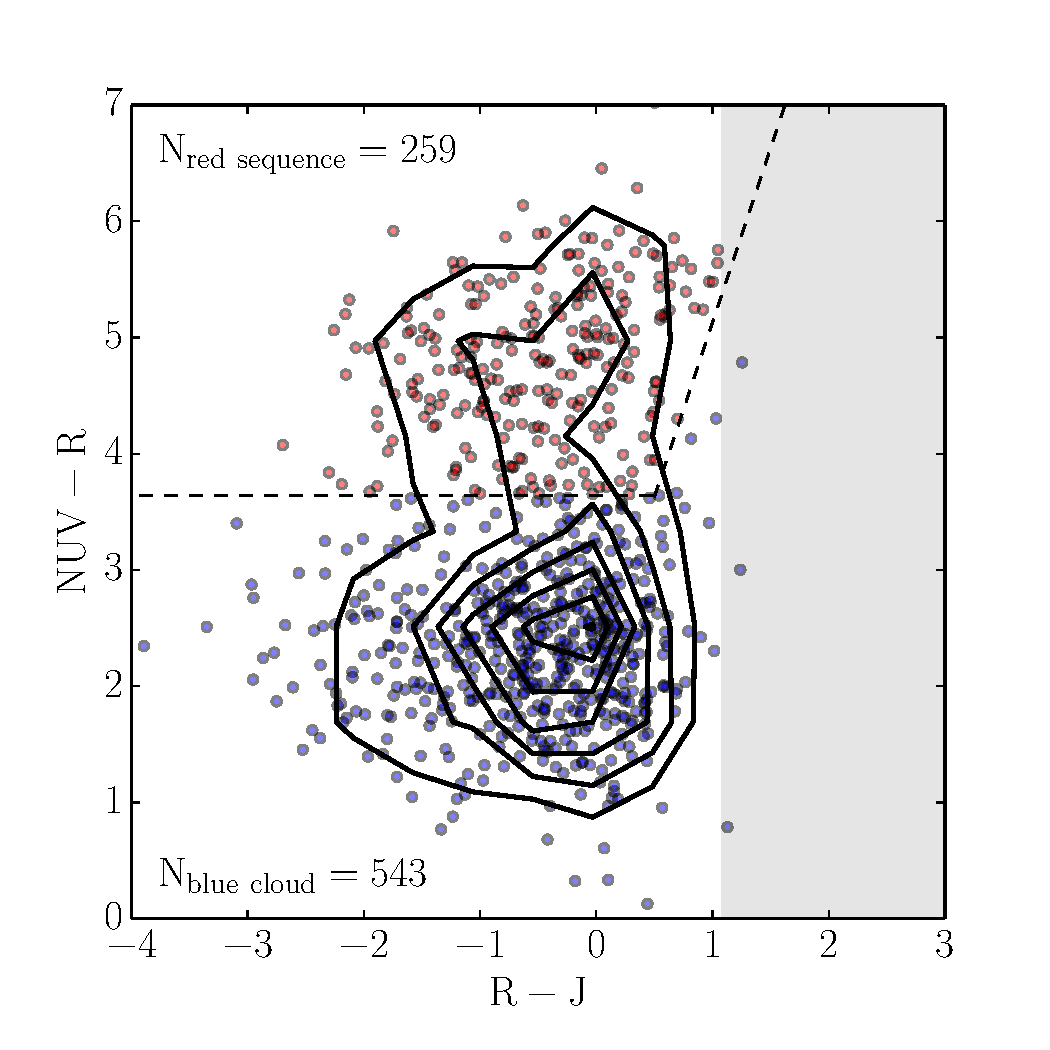
\includegraphics[width=2.5in,height=2.5in,trim={.5cm 0cm .5cm 0cm},clip]{figures/ferengi2_colorcolor.pdf}
\caption{Separation of the quiescent population (red sequence) and active population (blue cloud) of the \ferengi2 sample. The gray shaded region represents the R-J limit of the sample; since \ferengi2 is a subset of GZ2, for which a limit of $r<17$ was implemented, and the magnitude limit of 2MASS is $J<15.91$, the \ferengi2 sample is limited to R-J $<$ 1.1.}
\label{fig:ferengi2colorcolor}
\end{figure}

\begin{figure*}
\centering
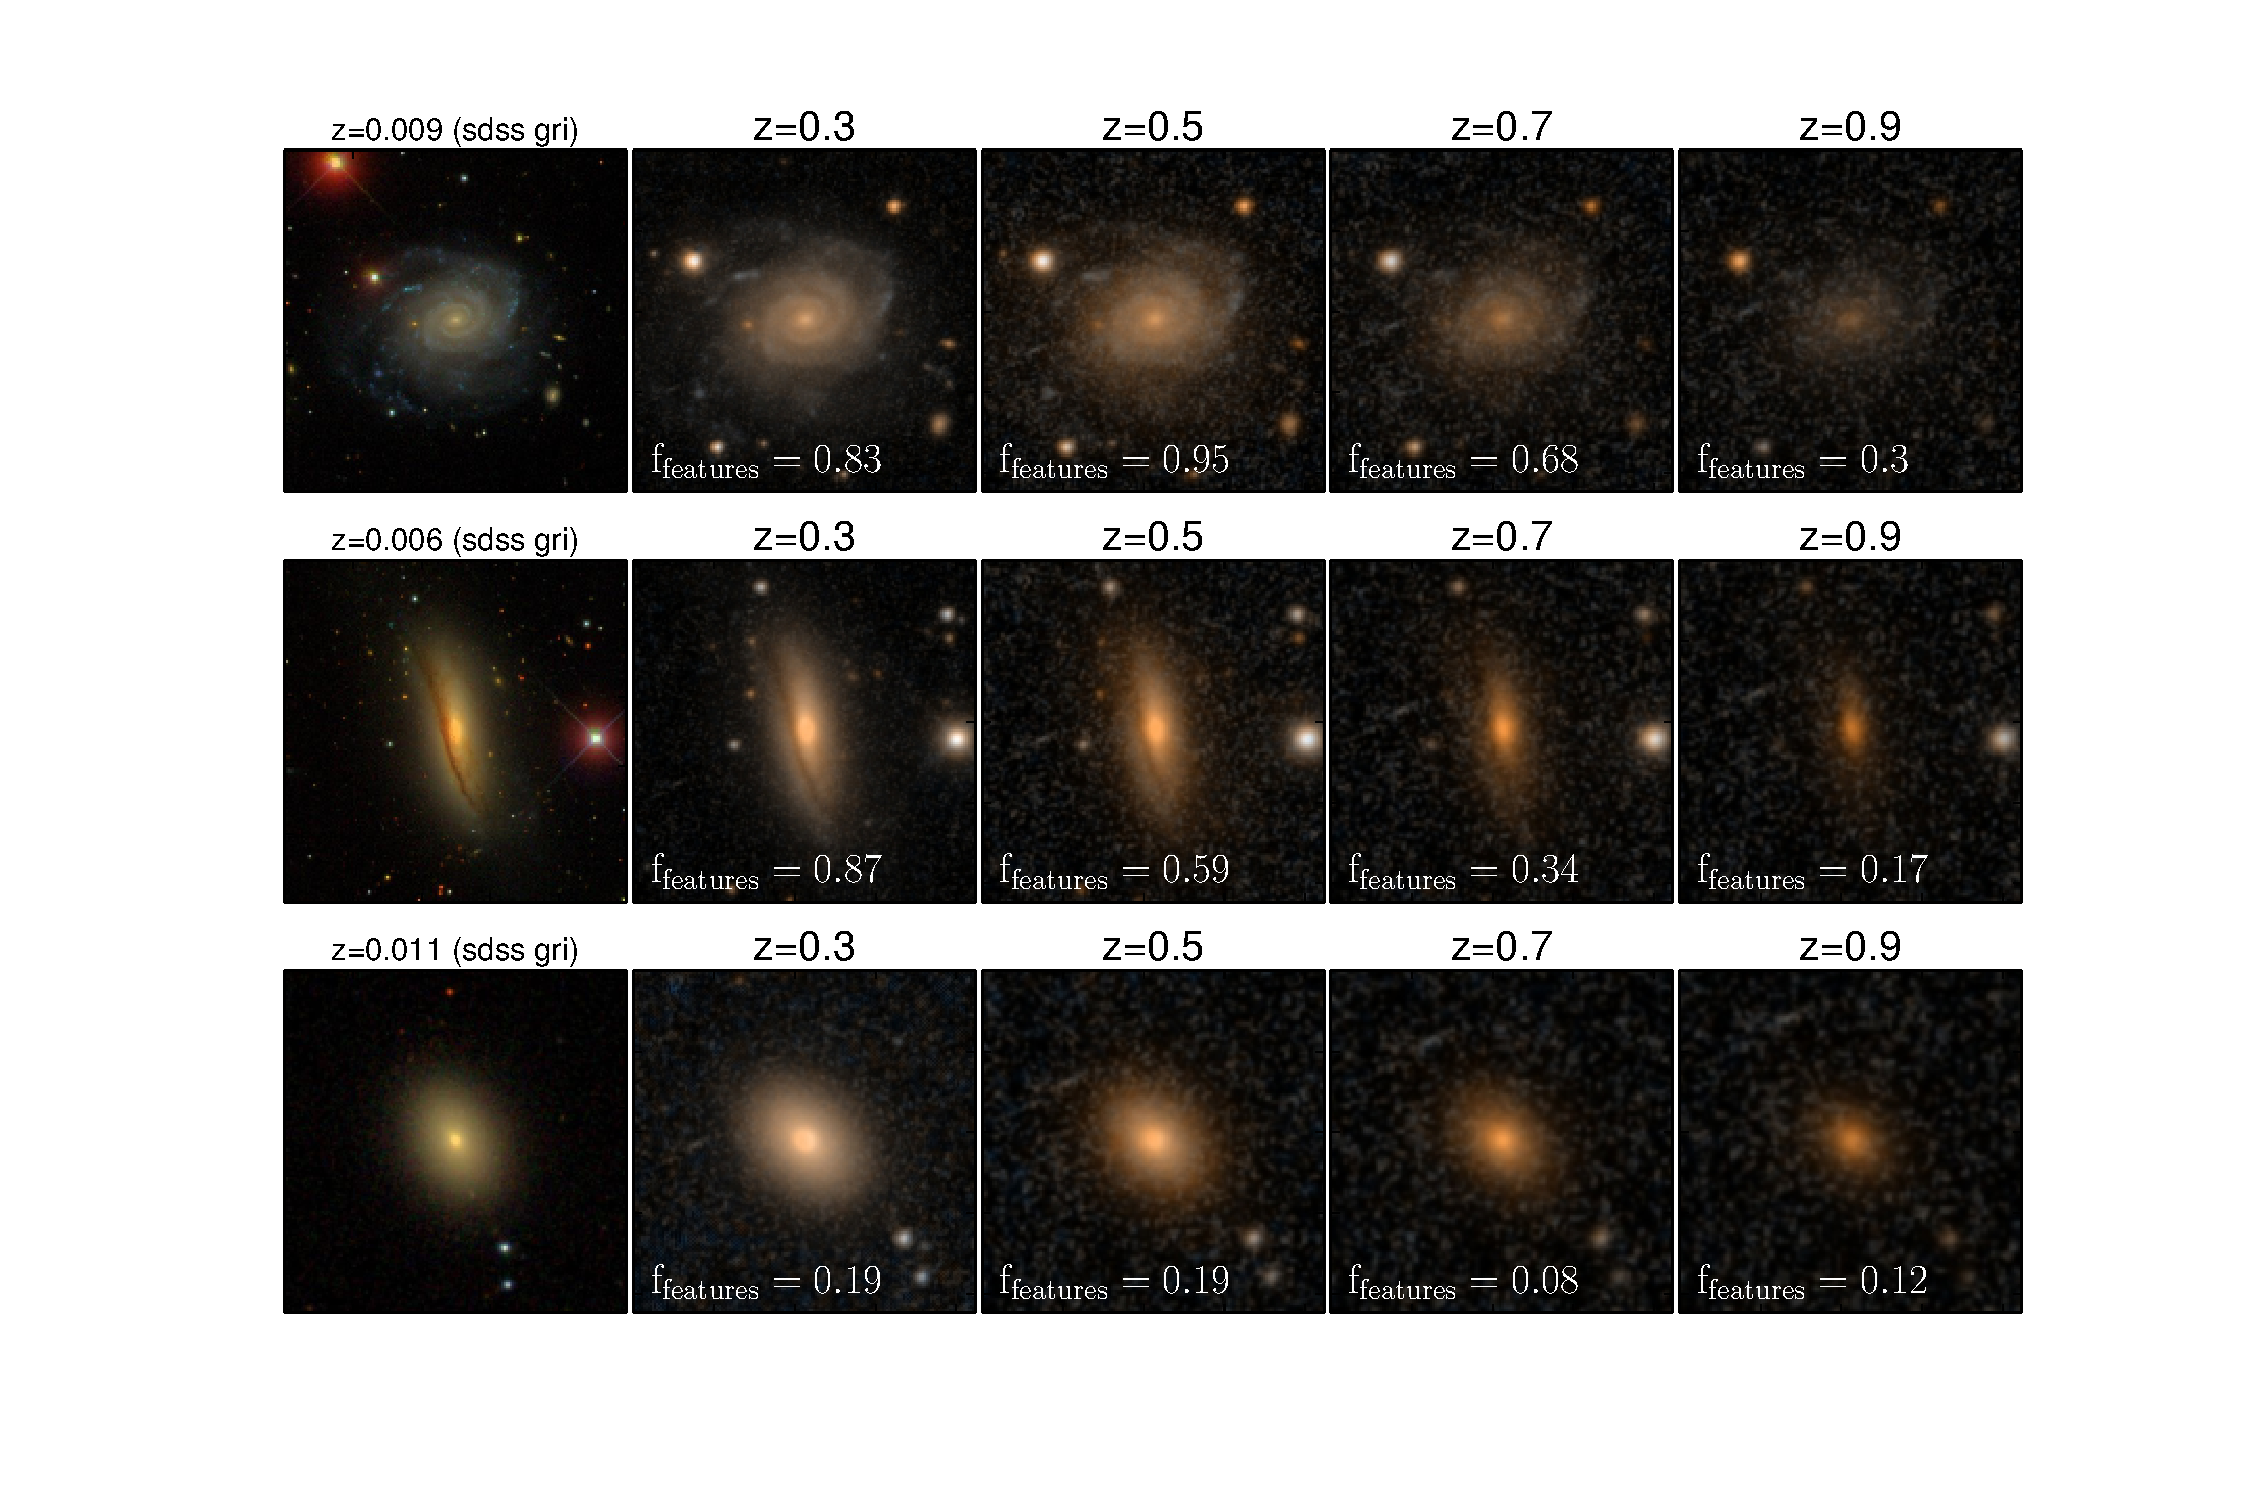
\includegraphics[width=\textwidth,trim={.5cm 3cm .5cm .5cm},clip]{figures/ferengi2_examples_with_fractions.pdf}
\caption{Example images of three galaxies artificially redshifted with the \ferengi{} code. The left image in each row is a real SDSS gri-composite image; the four to the right are images generated by \ferengi{} at varying redshifts, processed to mimic $HST/COSMOS$ imaging. The \ffeatures{} vote fraction for each simulated image is given; this value tends to decrease for each galaxy as it is processed to be viewed at higher redshifts. }
\label{fig:ferengi2example}
\end{figure*}

\subsection{Measuring the completeness in disc and elliptical detection, $\xi$}
\label{ssec:xi}

The \ferengi2 set was used to measure the incompleteness in disc and elliptical detection, from which correction factors $\xi_{disc}$ and $\xi_{ellitpical}$ were derived. These are defined as the number of discs/ellipticals detected divided by the true number of discs/ellipticals expected to exist in a given redshift interval: $\rm \xi_{disc}(z)=N_{discs~detected}/N_{\rm discs~true}$, and $\rm \xi_{elliptical}(z)=N_{ellipticals~detected}/N_{ellipticals~true}$


 Acknowledging that the completeness in disc detection may depend on galaxy colour, the corrected fraction of passive discs can then be calculated as:

\begin{equation}
f_{R|D}=\frac{N_{RD}\times \xi^{-1}_{red~discs}}{N_{RD}\times \xi^{-1}_{red~discs} + N_{BD} \times \xi^{-1}_{blue~discs}}
\label{eqn:fdir}
\end{equation}

If there is no colour bias in disc detection, $\xi_{red~discs}=\xi_{blue~discs}$, and this term cancels out, leaving the fraction unchanged. If there is a bias, however, the $\xi$ terms do not cancel, and the incompleteness in disc detection could have a large effect on the red disc fraction. Therefore a careful measurment of $\xi$ is estimated for both red and blue disc galaxies using the \ferengi2 set of simulated images. 

The completeness values $\xi_{red~discs}(z)$ and $\xi_{blue~discs}(z)$ were computed in varying bins of redshift for the red sequence and blue cloud galaxies separately. An example calculation of $\xi_{blue~discs}$ in the $z=0.7$ bin is shown in Figure~\ref{fig:inc_subplot}. Each point represents a \ferengi2 galaxy, where the y-axis indicates the value of \ffeatures~measured in the image redshifted to $z=0.7$, and the x-axis indicates the value of \ffeatures~measured in the same galaxy redshifted to $z=0.3$. Disk galaxies are identified as those for which \ffeatures~$\ge0.3$. Since, on average, \ffeatures~decreases for the same galaxy as it is viewed at higher redshifts, the number of galaxies meeting this threshold is generally fewer at higher redshifts than lower redshifts. This is indicated by the dotted lines: galaxies to the right of the vertical dashed line at $\rm f_{features,z=0.3}=0.3$ are identified as discs at $z=0.3$; their sum is considered the ``true'' number of discs, $\rm N_{true}$. Similarly, the galaxies above the horizontal line at $\rm f_{features,z=0.7}=0.3$ are identified as discs at $z=0.7$; their sum is the ``detected'' number of discs at $z=0.7$, or $\rm N_{discs~detected}$. As obvious in the figure, $\rm N_{discs~detected}$ is in general much lower than $\rm N_{discs~true}$, emphasizing the increasing difficulty in detecting features at higher redshifts. Their ratio is the completeness $\xi$; in this example $\xi_{blue~discs}(z=0.7)=0.61$, meaning only 61\% of discs were detected at this redshift. 

\begin{figure}
\centering
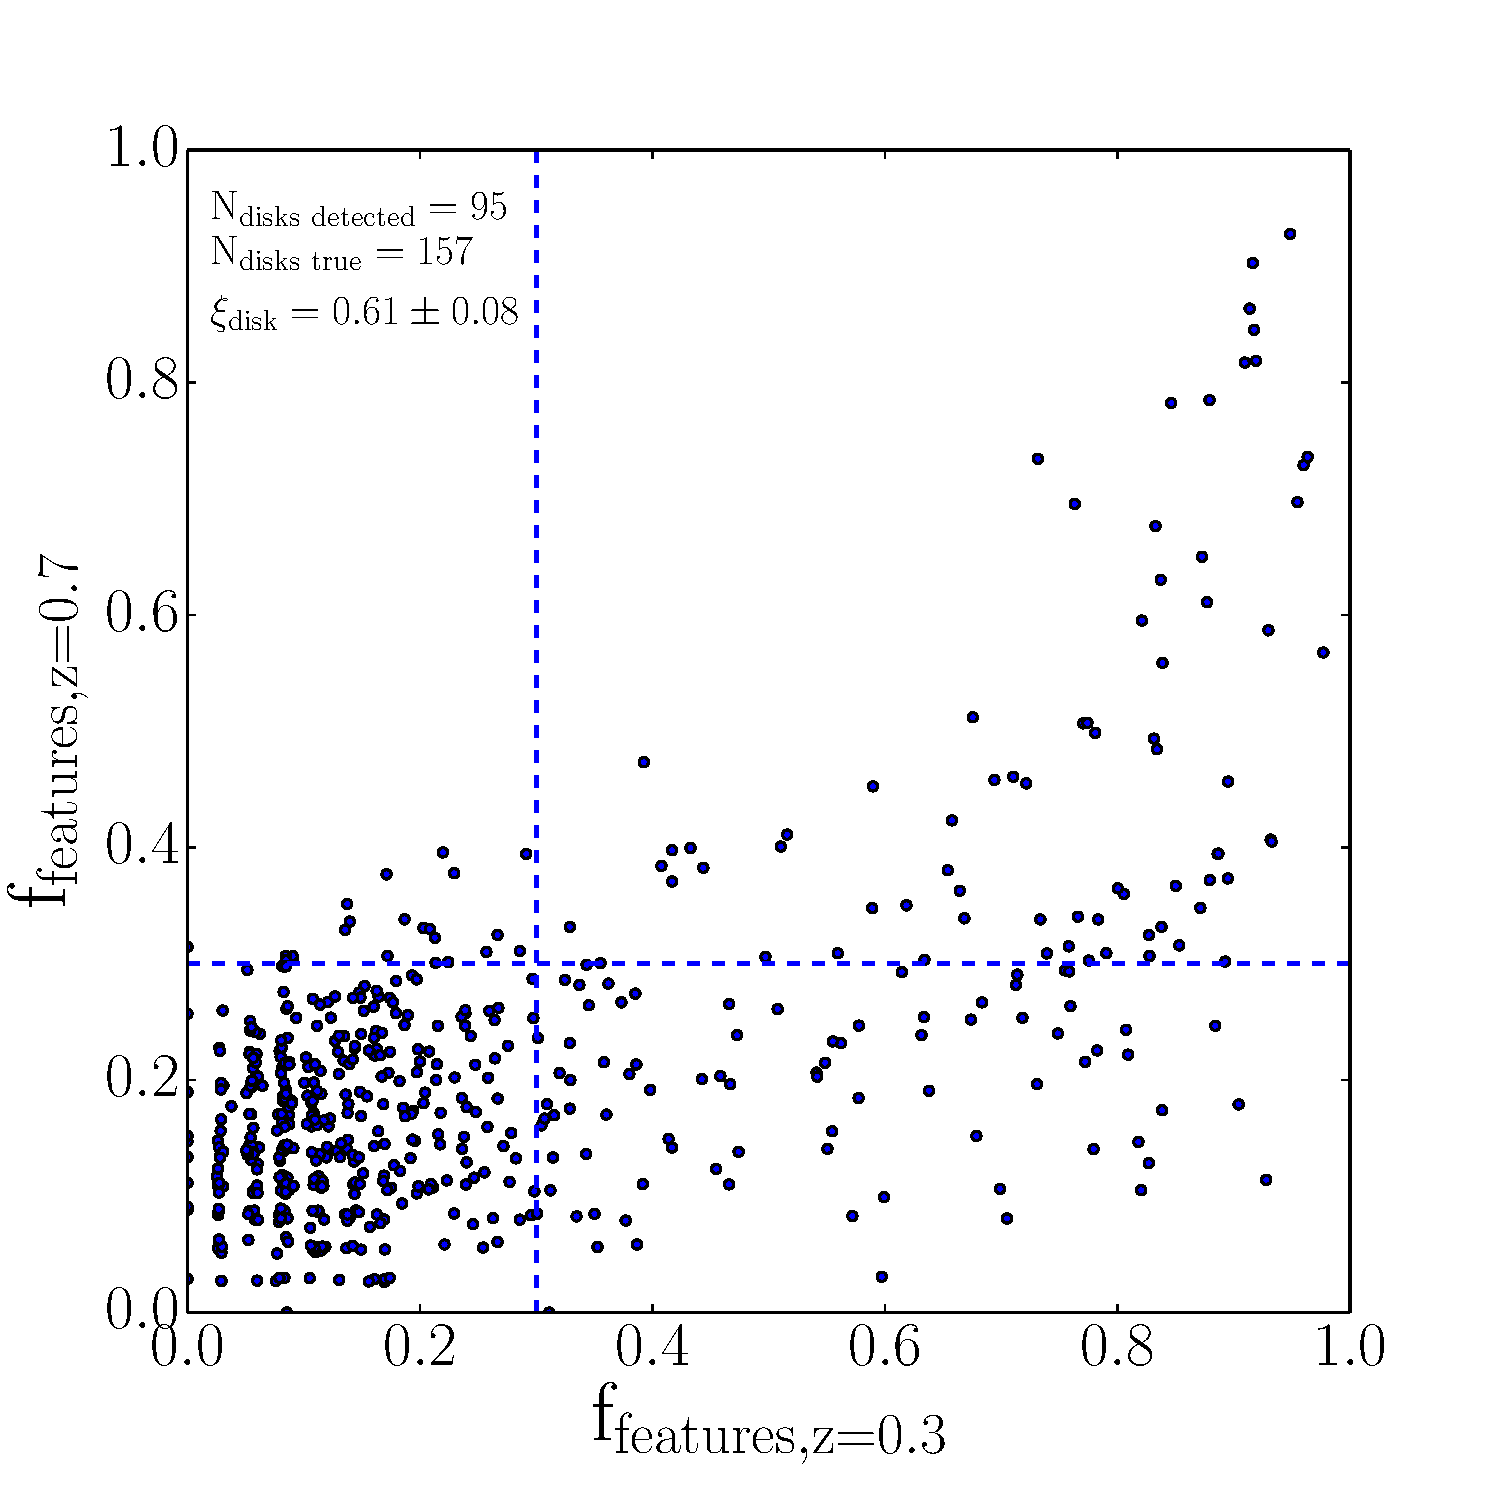
\includegraphics[width=.4\textwidth]{figures/incompleteness_z7.pdf}
\caption{Example calculation of completeness $\xi_{disc}$ at redshift $z=0.7$. Points represent \ferengi2 images classified in Galaxy Zoo. The y-axis corresponds to the value of \ffeatures~measured at the galaxy redshifted to $z=0.7$, and the x-axis corresponds to the value of \ffeatures~measured at the galaxy redshifted to $z=0.3$. On average, the \ffeatures~is lower at the higher redshift, indicating users on average have more difficulty identifying features in images at higher redshifts. The dotted lines correspond to \ffeatures=0.3, the threshold above which a galaxy is considered to have a disc. Galaxies to the right of the vertical dashed line were identified as discs at the lowest redshift $z=0.3$, the total number defined as $\rm N_{discs~true}$, the true number of discs. Galaxies above the horizontal dash line were identified as discs at the higher redshift $z=0.7$, the total number defined as $\rm N_{discs~detected}$. The ratio $\rm \xi_{disc}=N_{discs~detected}/N_{discs~true}$ is the completeness value; in this example, only 61\% of discs were detected at $z=0.7$.}
\label{fig:inc_subplot}
\end{figure}

It was hypothesized that the completeness in disc detection may be a function of other parameters in addition to redshift. At fixed redshift, for example, it is reasonable to guess that features could be easier to detect galaxies that have higher mass, radius, or surface brightness. To test whether these parameters also impact the number of discs detected, the completeness was measured in fixed redshift bins as a function of surface brightness, effective radius, and mass. The surface brightness was calculated as $\mu = m + 2.5*\log_{10}{(2 \times (b/a) \times \pi R_e^2 )}$, using \sextractor{} outputs {\tt MAG\_AUTO}, $b/a$ and $R_{e}$ measured in the \Iband{} band images. The effective radius used was the 50\% {\tt FLUX\_RADIUS} converted in to kpc, and the masses used were the {\tt MEDIAN} values in the MPA-JHU DR7 catalog \citep{Kauffmann2003b}.

Figure~\ref{fig:xi_v_sb} shows completeness as a function of redshift and surface brightness, for the red sequence and blue cloud disc galaxies. 8 redshift bins were further divided into bins of surface brightness with varying widths, where the sizes were chosen to satisfy that $\rm N_{discs~detected} + N_{discs~true} \ge 10$ in each bin. This was chosen as a compromise between having a sufficient number of galaxies in each bin to compute the completeness fraction $\rm \xi_{disc} = N_{discs~detected}/N_{discs~true}$, and to have enough bins of surface brightness to measure a trend with confidence of completeness as a function of $\mu$. Visual inspection of the data did not suggest any relationship between the two. To be sure, the data were fit to a linear function in each redshift bin. For each fit, a p-value representing a hypothesis test whose null hypothesis is that the slope is zero was computed. Only one reached the criteria $p<0.05$, but with a low $R^{2}$ value of 0.28 which is not considered large enough to represent a good fit. This process was repeated using effective radius and mass as parameters, and for the elliptical galaxies in the computation of $\xi_{elliptical}$, with the same results. Therefore only redshift was used as a parameter which impacted completeness values with confidence. 

\begin{figure}
\centering
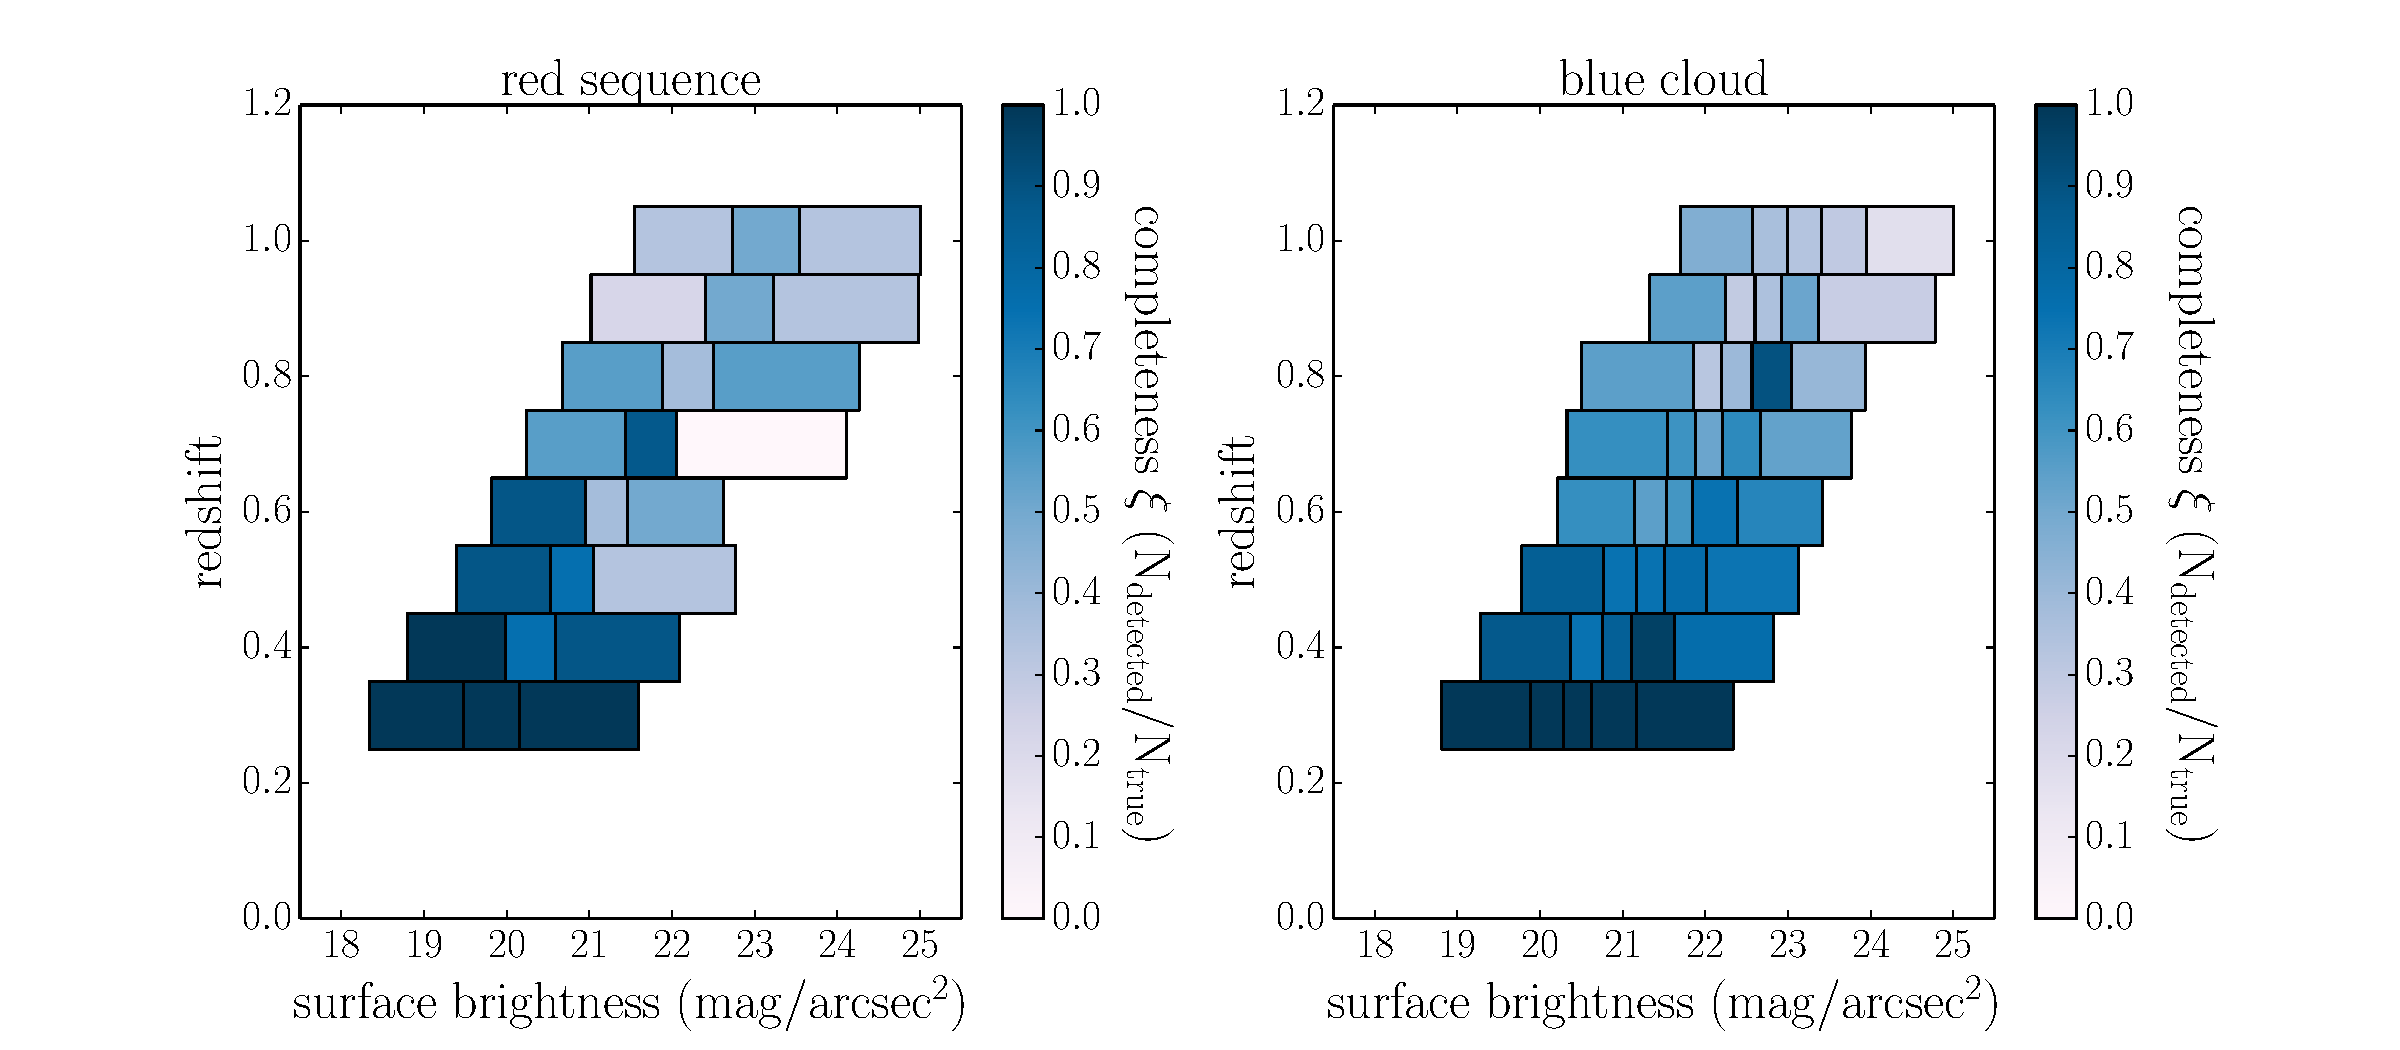
\includegraphics[width=3.5in,trim={3cm 0cm 3cm 0cm},clip]{figures/xi_v_sb.pdf}
\caption{Completeness $\xi_{disc}$ as a function of redshift and surface brightness for red sequence (left) and blue cloud galaxies (right). In each redshift bin, galaxies were binned by surface brightness in varying widths such that $\rm N_{discs~detected} + N_{discs~true} \ge 10$ in each bin. The completeness values $\xi_{disc}$ )and $\xi_{elliptical}$, not displayed) were computed in each $z,\mu$ bin, represented by the colours. Darker colours represent a completeness of 1, such that all discs were detected, while fainter colours represent a completeness near 0, representing a failure to detect discs. $\xi_{disc}$ tends to decrease with redshift, but no correlation of $\xi_{disc}$ with surface brightness is observed at fixed redshift.}
\label{fig:xi_v_sb}
\end{figure}


The completeness values $\rm \xi_{red~discs}$ and $\rm \xi_{blue~discs}$ were then measured as a function of redshift for the red sequence and blue cloud \ferengi2 galaxies; results are shown in Figure~\ref{fig:xi}. No significant difference was detected for the two functions, which is apparent from the overlapping $1-\sigma$ errors on the plot. The process was then repeated for the elliptical galaxies; as with the disc sample, no dependence on completeness $\xi_{elliptical}$ with variables other than redshift was found. Therefore $\xi_{disc}$ and $\xi_{elliptical}$ were computed for all galaxies in bins of redshift between 0.3 and 1.0 with widths $\Delta z = 0.1$; from here linear relationships for $\xi_{disc}$ and $\xi_{elliptical}$ as functions of redshift were derived: $\xi_{disc}(z) = -0.97 \pm 0.04 (z) + 1.29 \pm 0.02$, $\xi_{elliptical}(z) = 0.32 \pm 0.02 (z) + 0.90 \pm 0.01$. These corrections were used to calculate the fractional contribution of each morphological/activity type (Figure~\ref{fig:all_plot}), and the fraction of discs on the red sequence (Figure~\ref{fig:f_results}):

\begin{equation}
f_{D|R}=\frac{N_{RD}\times \xi_{disc}^{-1}}{N_{RD}\times \xi_{disc}^{-1} + N_{RE}\times \xi_{elliptical}^{-1}}
\label{eqn:frid}
\end{equation}


\begin{figure}
\centering
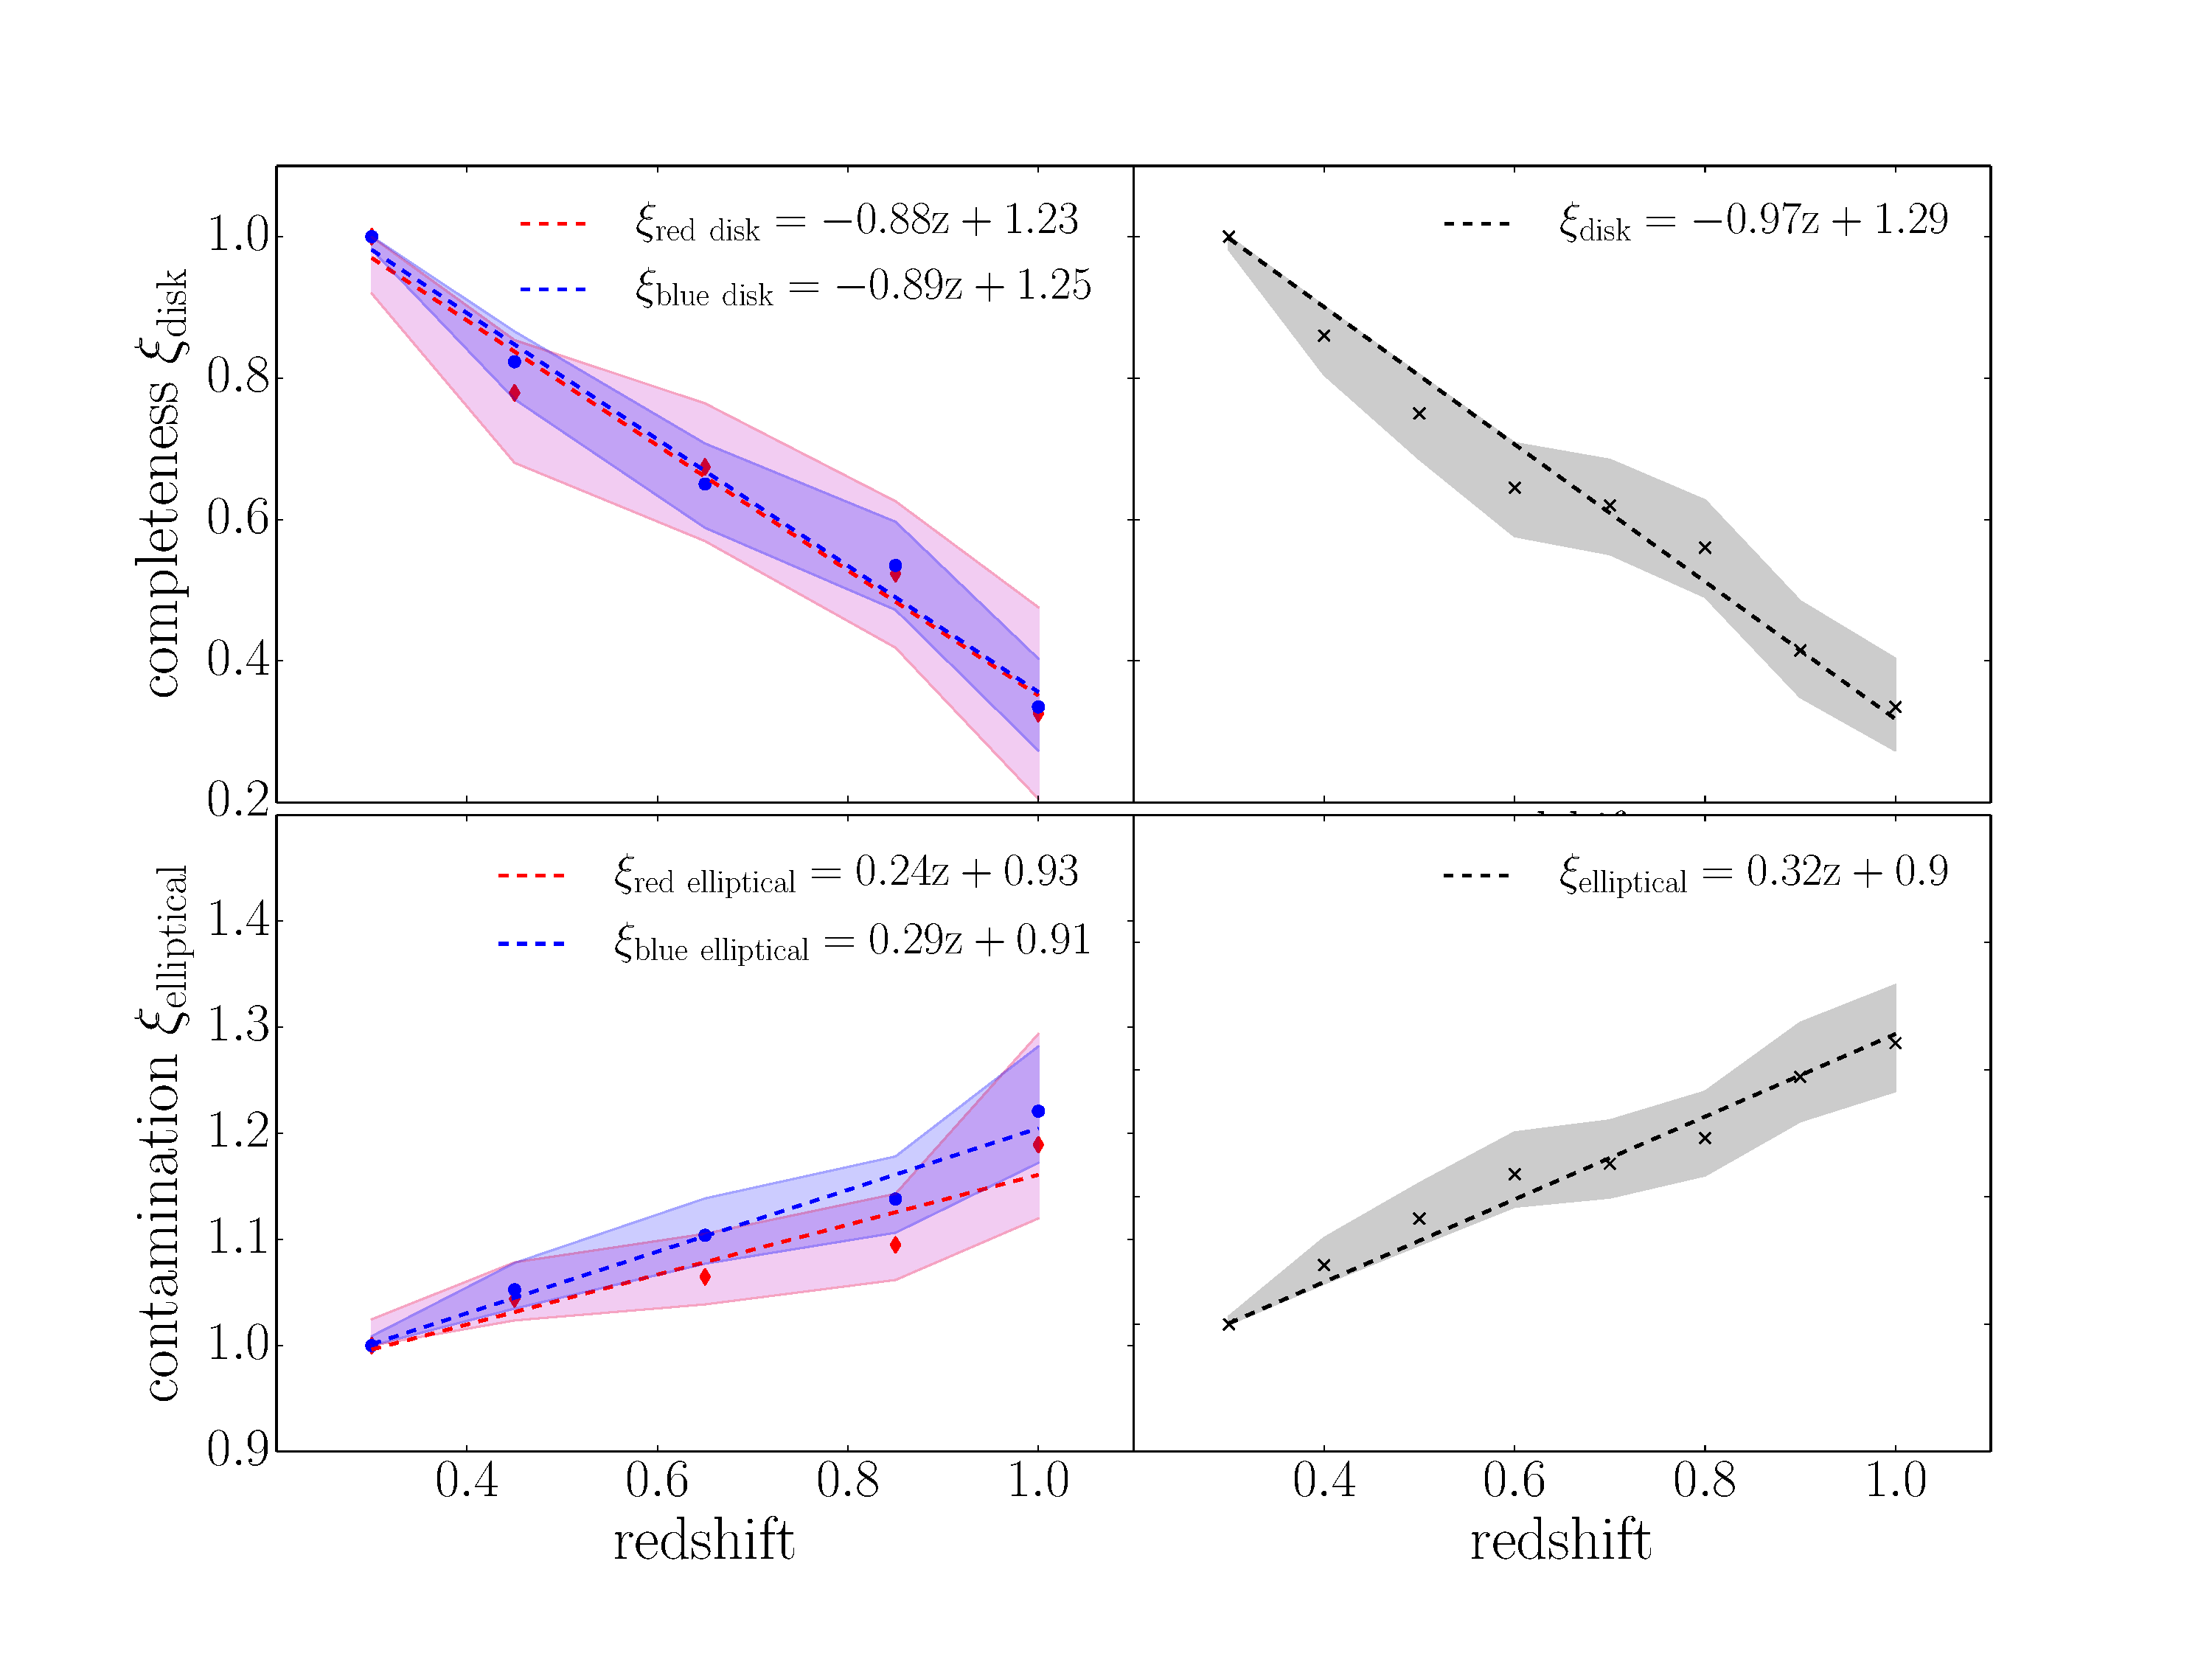
\includegraphics[width=0.5\textwidth,trim={3cm 1.5cm 3cm 3cm},clip]{figures/completeness_full.pdf}
\caption{\textbf{Left:} Completeness $\xi_{disc}$ (top) and $\xi_{elliptical}$ (bottom) as a function of redshift for red sequence and blue cloud \ferengi2 galaxies separately. All show a clear dependence on $\xi$ with redshift, but there is no strong difference in completeness for the red and blue populations. \textbf{Right:} Completeness $\xi_{disc}$ (top) and $\xi_{elliptial}$ (bottom) as a function of redshift for all  \ferengi2 galaxies (red and blue combined). The equation representing the linear fit for each is displayed.}
\label{fig:xi}
\end{figure}

\section{Results}
\label{sec:results}
In this section we present our results for the evolution of the fraction of star-forming and quenched disc and elliptical galaxies from $z=1$ to $z=0.3$ in a sample of 20,811 $COSMOS$ galaxies morphologically classified in GZH. In Figure~\ref{fig:all_plot}, we divide our sample into four bins of galaxy stellar mass and plot how the fractional contributions of all four colour-morphology permutations vary as a function of redshift.  Using the same binning of our parent sample in $M_*-z$ space, equations 3 (left-panel) and 4 (right panel) were evaluated for each subsample to yield the curves that are plotted in Figure~\ref{fig:f_results}. In discussing these results, we refer to increases/decreases in these fractions with respect to \emph{increasing} cosmic time; that is, from right to left in the plots shown in Figures~\ref{fig:all_plot}\ref{fig:f_results}.

\begin{figure*}
\centering
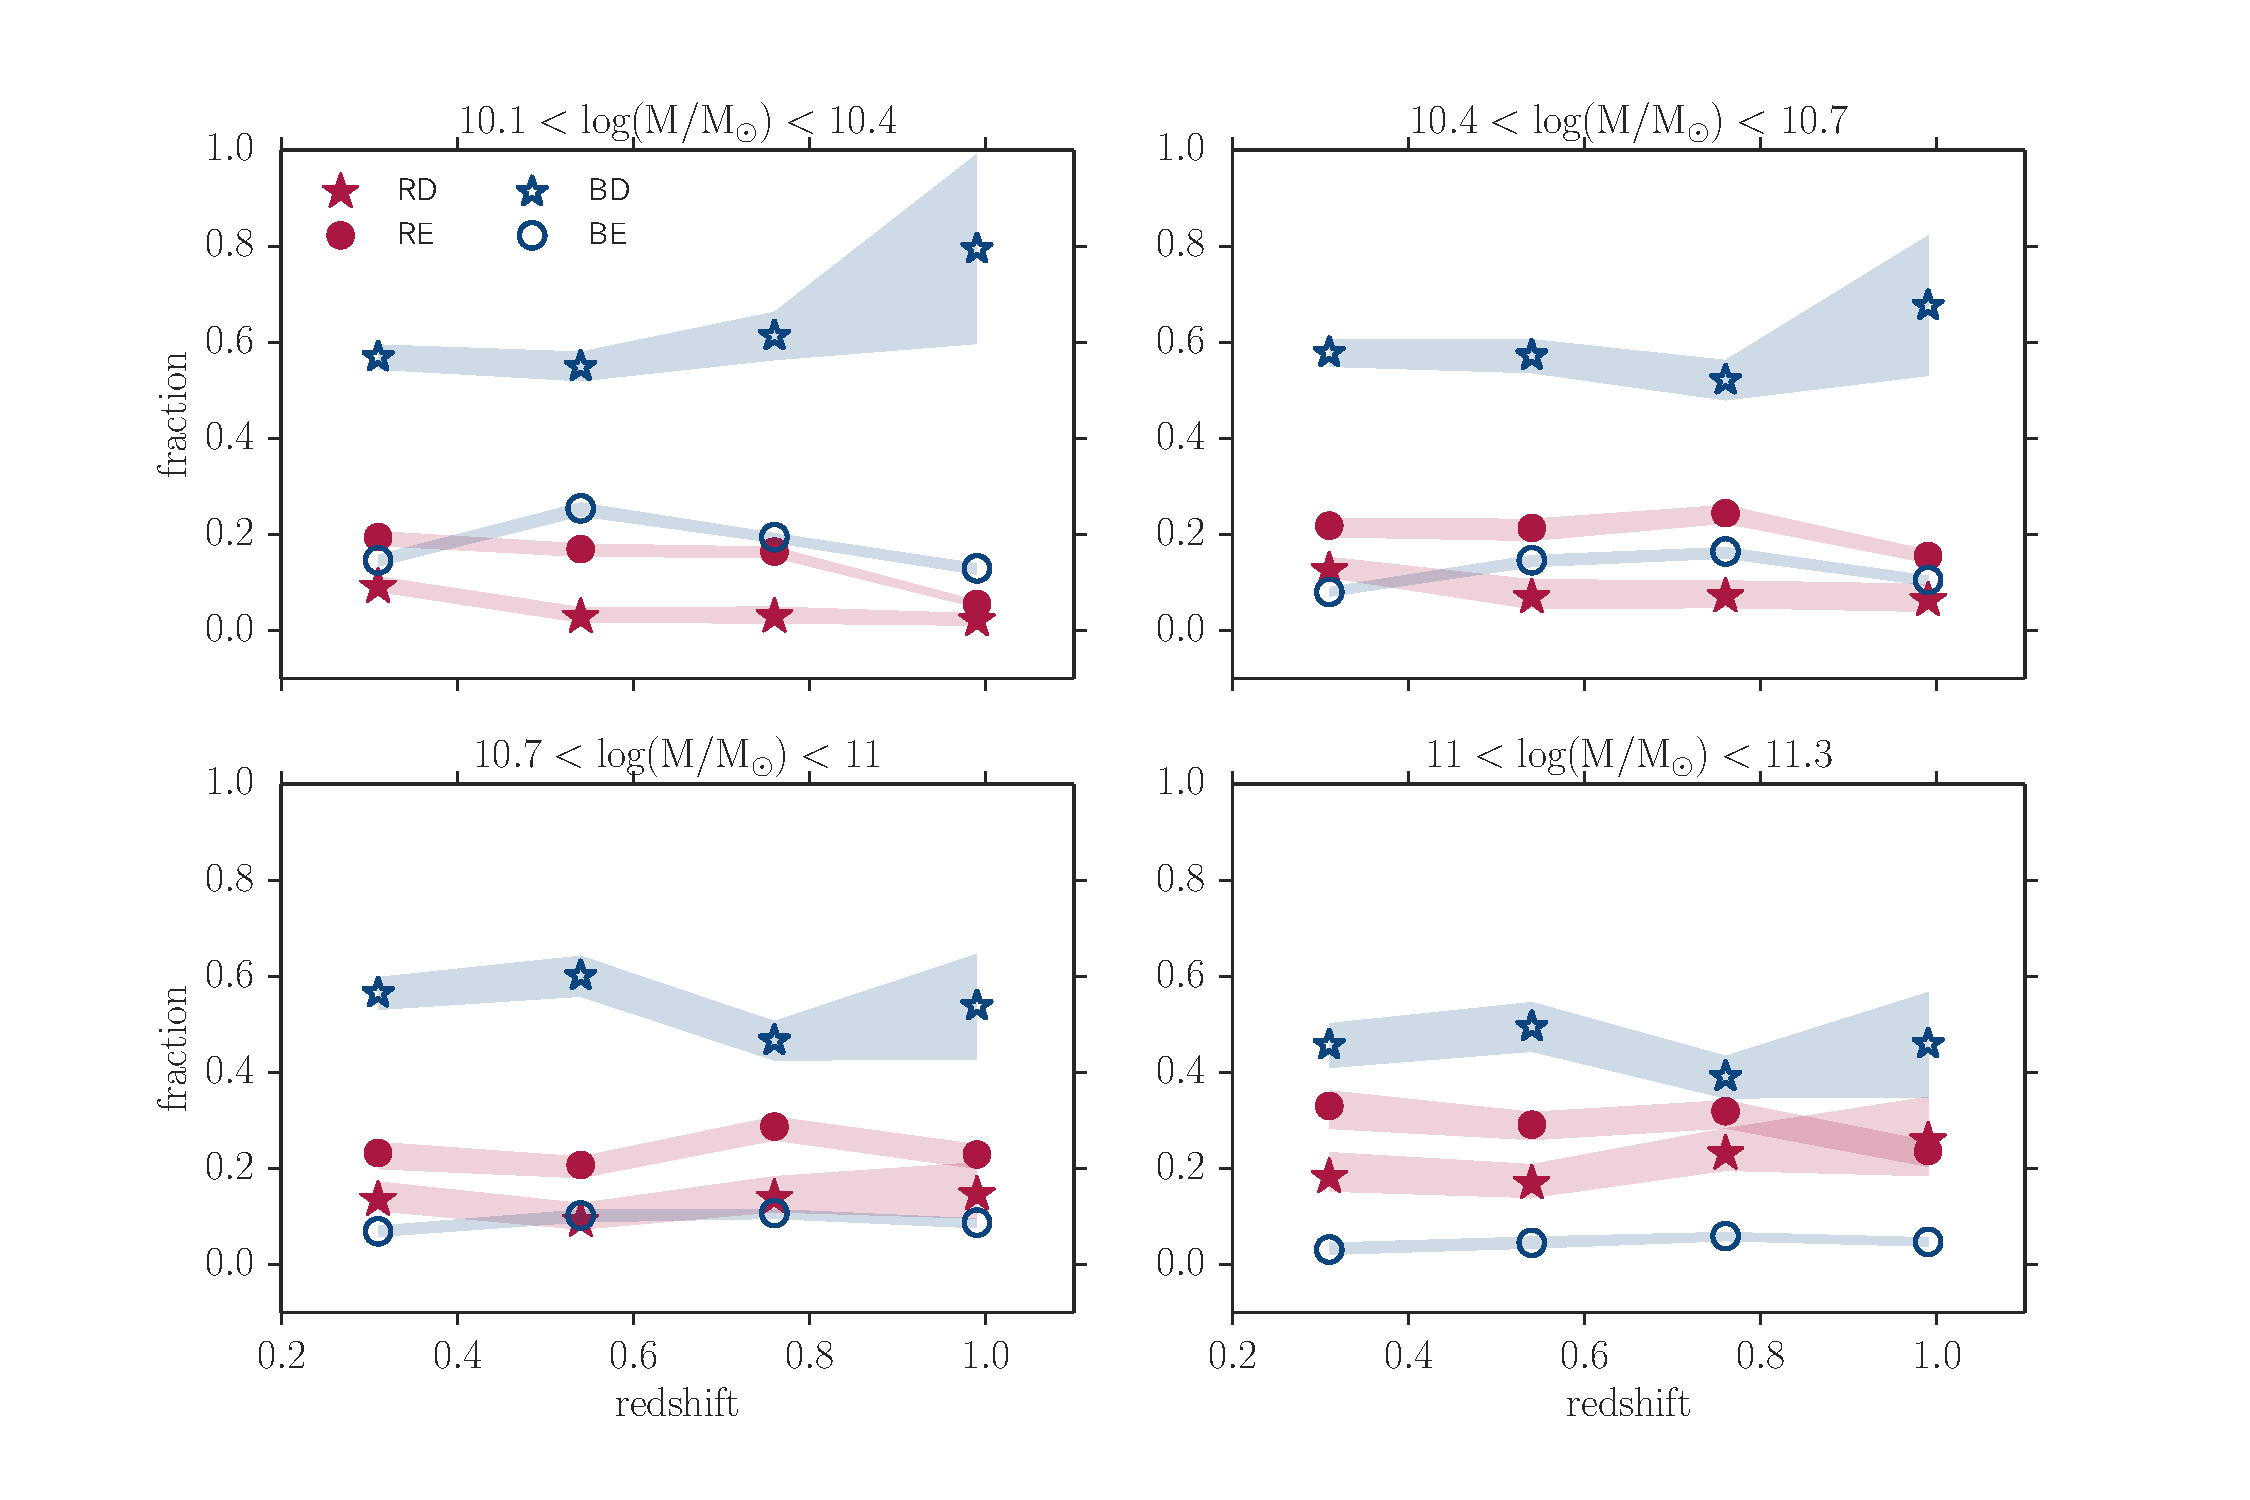
\includegraphics[width=\textwidth,trim={0cm 0cm 2cm 1cm},clip]{figures/morphologies_evolved.pdf}
\caption{Evolution of four types of galaxy populations since $z=1$: blue discs (blue open stars), red discs (red closed stars), blue ellipticals (blue open circles), and red ellipticals (red closed circles). Each point represents the fraction of the indicated type with respect to the total population, such that all points in a given redshift, mass bin sum to 1. Errors on each fraction are indicated by the shaded regions, and are propagations of $\sqrt{N}$ counting errors and the errors associated with the functional fits to the correction terms $\xi_{\rm disc}$ and $\xi_{\rm elliptical}$ (Section~\ref{ssec:xi}). }
\label{fig:all_plot}
\end{figure*}


\begin{figure*}
\centering
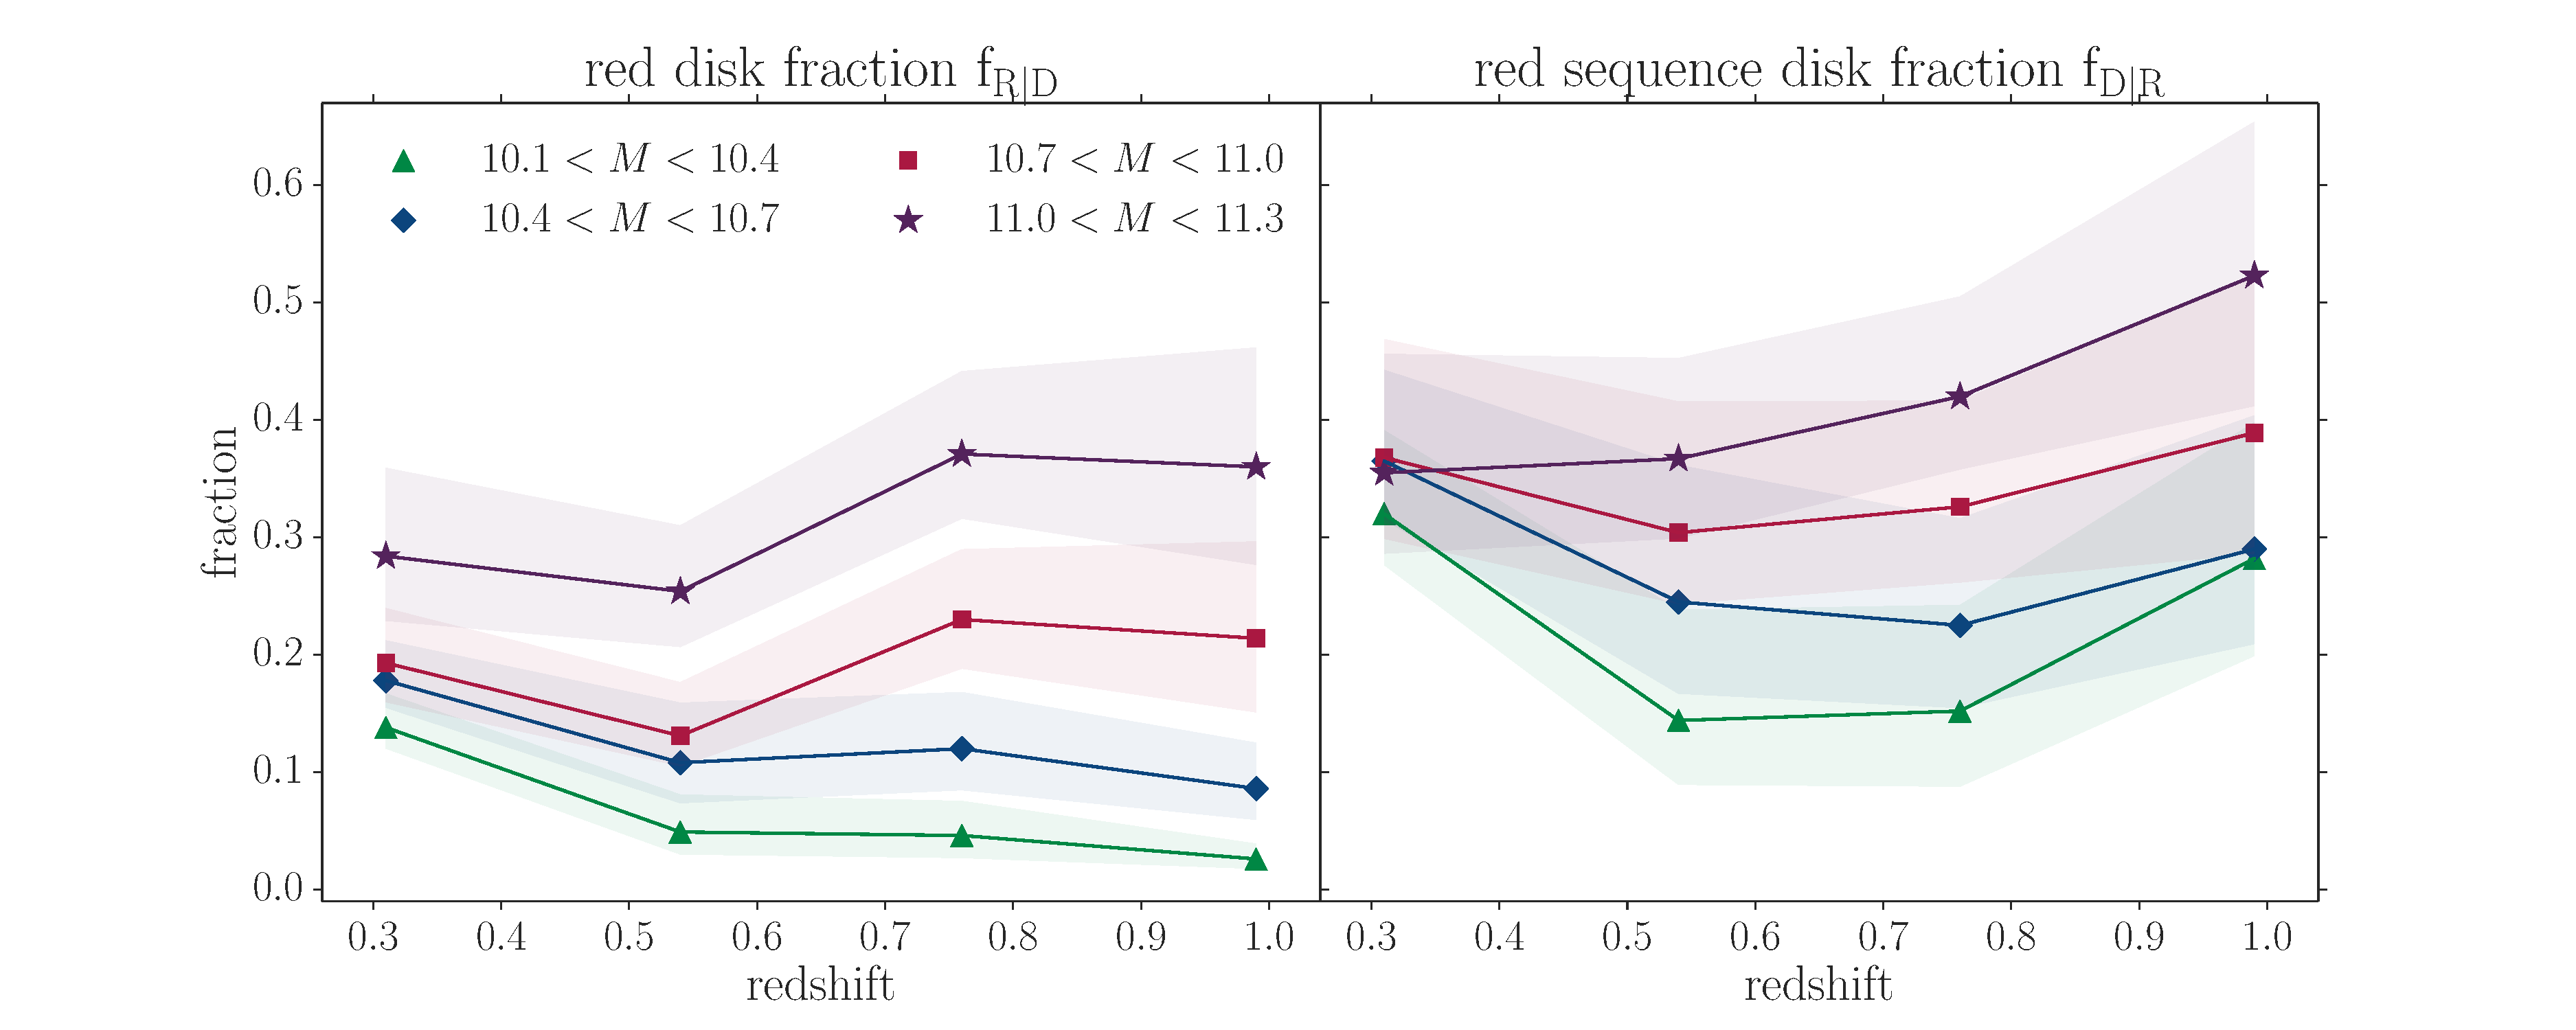
\includegraphics[width=\textwidth,trim={0cm 0cm 2cm 1cm},clip]{figures/red_disk_fractions.pdf}
\caption{\textbf{Left:} Passive disc fraction ($\rm N_{red~discs}/(N_{red~discs}+N_{blue~discs})$) vs redshift in four mass bins. \textbf{Right:} Fraction of discs on the red sequence ($\rm N_{red~discs}/(N_{red~discs}+N_{red~ellipticals})$) vs redshift in four mass bins. Errors on each fraction are indicated by the shaded regions, and are propagations of $\sqrt{N}$ counting errors and the errors associated with the functional fits to the correction terms $\xi_{\rm disc}$ and $\xi_{\rm elliptical}$ (Section~\ref{ssec:xi}).} 
\label{fig:f_results}
\end{figure*}


%super basic: absolute numbers
In Figure~\ref{fig:all_plot} we find blue discs are the plurality population at each redshift for all mass bins. At fixed redshift, the abundance of the red disc population is maximised in the highest mass bin and decreases monotonically towards lower masses. Red ellipticals tend to significantly outnumber red discs except in the highest mass/redshift bin, where the population sizes are almost equal. Blue ellipticals represent an insignificant fraction for galaxies with mass $\rm log(M/M_{\odot})>10.7$, but begin to outnumber the red disc population at lower masses. 

%next: trends
%explain SF?

%trends
Red disc galaxies are presumed to form primarily from blue discs galaxies which have quenched without undergoing a morphological transformation. If this is true, and if the resulting quenched discs do not continue in their evolution, one would expect a ``pile up'' of red discs at later times, resulting in an increasing fraction at lower redshift. This trend is observed in the two lowest mass bins, however there is no large change in the fractional contribution of red disks to the total population in the $\rm log(M/M_{\odot})\sim10.85$ bin, and even a small decrease in the highest mass bin. If we assume that red discs are continuously produced from blue discs, even at a small rate, then a constant or decreasing fraction can only be explained if their numbers are simultaneously being depleted, presumably by a morphological transformation to red elliptical.

The evolution of the red disc population is more apparent in Figure~\ref{fig:f_results}.  The left panel shows the red disc fraction, the ratio of red discs to all discs ($f_{\rm R|D} = \rm N_{\rm red~discs}/(N_{\rm red~discs}+N_{\rm blue~discs}))$. The right panel shows the red sequence disc fraction, the ratio of red discs to all red sequence galaxies ( $f_{\rm D|R} = \rm N_{\rm red~discs}/(N_{\rm red~discs}+N_{\rm red~ellipticals}))$. We observe a mass-dependence in both fractions. At fixed redshift, both $f_{R|D}$ and $f_{D|R}$ tend to increase with increasing mass; this is a consequence of the higher abundance of red discs observed at high masses, as seen in Figure~\ref{fig:all_plot}. 

Given the large errors on some of the fractions (particularly for $f_{D|R}$), we check whether $f_{R|D}$ and $f_{D|R}$ increase, decrease, or remain constant as functions of redshift in each mass bin by fitting the data to a linear function and evaluating if their slope is consistent with zero, defined as such if zero exists within the $1 \sigma$ errors on the slope. We find that the red disc fraction $f_{R|D}$ decreases for the highest mass bin, is constant for $\rm log(M/M_{\odot})~10.85$, and increases for the two lower mass bins $\rm log(M/M_{\odot})<0.7$. An increase in $f_{R|D}$ could be driven by the increase of red discs or a depletion of blue discs; Figure~\ref{fig:all_plot} shows the increase may be driven more from the latter at $z\sim1$, and the former at lower redshift. On the right, we find a decrease in the red sequence disc fraction $f_{D|R}$ for all masses in the interval from $z\sim1$ to $z\sim0.8$. Figure~\ref{fig:all_plot} shows that this is mainly driven by the increase in red ellipticals during this time, which is consistent with higher merger rates at this epoch \citep{Molina2016}. From $z\sim0.8$ to $z\sim0.3$, $f_{D|R}$ continues to decrease for galaxies $log(M/M_{\odot})>11$, becomes constant for galaxies $\rm log(M/M_{\odot})\sim10.85$, and increases for the lower mass bins. Figure~\ref{fig:all_plot} reveals that the enhancement of $f_{D|R}$ among the low mass population is driven more by increases in the proportion of red discs, and rather than a depletion of red ellipticals. The increase of $f_{R|D}$ and $f_{D|R}$ with redshift observed at low masses, coupled with the constant or decreasing trends for high masses, suggests that low mass red disc galaxies may be more likely to remain as such, while more massive red disc galaxies are more likely to evolve further via a morphological transformation. We explore the potential drivers of these trends in terms of different evolutionary quenching pathways in detail in Section~\ref{sec:discussion}.

The downward trend we observe in the red sequence disc fraction $f_{D|R}$ for massive galaxies is in agreement with \citet{Bundy2010} (hereafter B10) who perform a similar analysis of the morphological makeup of the red sequence. As stated previously, a downward trend of $f_{D|R}$ represents either a depletion of the total pool of red discs (via a transformation to elliptical), but could also be an indication of an increase in the pool of red ellipticals (which could result from blue or red discs transforming morphology). In contrast, an upward trend is only possible via a pile-up of red discs, which is what we observe for the lower mass bins, and is in disagreement with B10. At the lowest redshift bin ($z\sim0.3$), we measure similar absolute fractions of discs occupying the red sequence for all masses. However, B10 find the contribution of low mass galaxies to increase at higher lookback time to $z=1$, while we find a decreasing contribution. 

The fact that our results agree for the highest mass at all redshifts, but only at the lowest redshift for lower masses, suggests the differences may be attributed in biases in morphological classification. B10 segregates early and late-type disc galaxies using ZEST \citep{Scarlata2007} morphologies, which they acknowledge are biased towards disc classification for faint apparent magnitudes, which tend to be associated with the lowest mass, highest redshift objects. This bias could influence their observed increase in red sequence discs toward $z=1$ for low masses. Conversely, GZ classifications tend to be biased towards elliptical morphologies at fainter magnitudes. Our attempt to quantify and correct for this effect is described in Section~\ref{ssec:ferengi}, but an underestimation of our correction function may have driven the apparently decreasing abundance of disc galaxies observed at increasing redshift for low masses. However, it has been shown that red disc galaxies in the local Universe tend to be more massive, as in \citet{Masters2011}. If this is true at all epochs, we would not expect such a significant contribution by red discs to the low-mass galaxy population as found in B10.

\section{Discussion}
\label{sec:discussion}
%first: reiterate what was done and with main conclusions/points drawn. 
We have examined the evolution of red disc galaxies since $z=1$ in Figures~\ref{fig:all_plot} and~\ref{fig:f_results}. Different trends in the abundance of red discs for distinct stellar mass bins are observed, which are consistent with a physical scenario in which 1) more massive galaxies undergo morphological transformations to elliptical at a higher rate than their less massive counterparts (implied by the decrease/increase of $f_{D|R}$ from $z=1$ to $z=0.3$ for high/low mass bins), and 2) more massive galaxies are more likely to enter a red disc phase to begin with (implied by the higher proportion of red discs in the high mass bin of Figure~\ref{fig:all_plot}). 

\begin{figure}
\centering
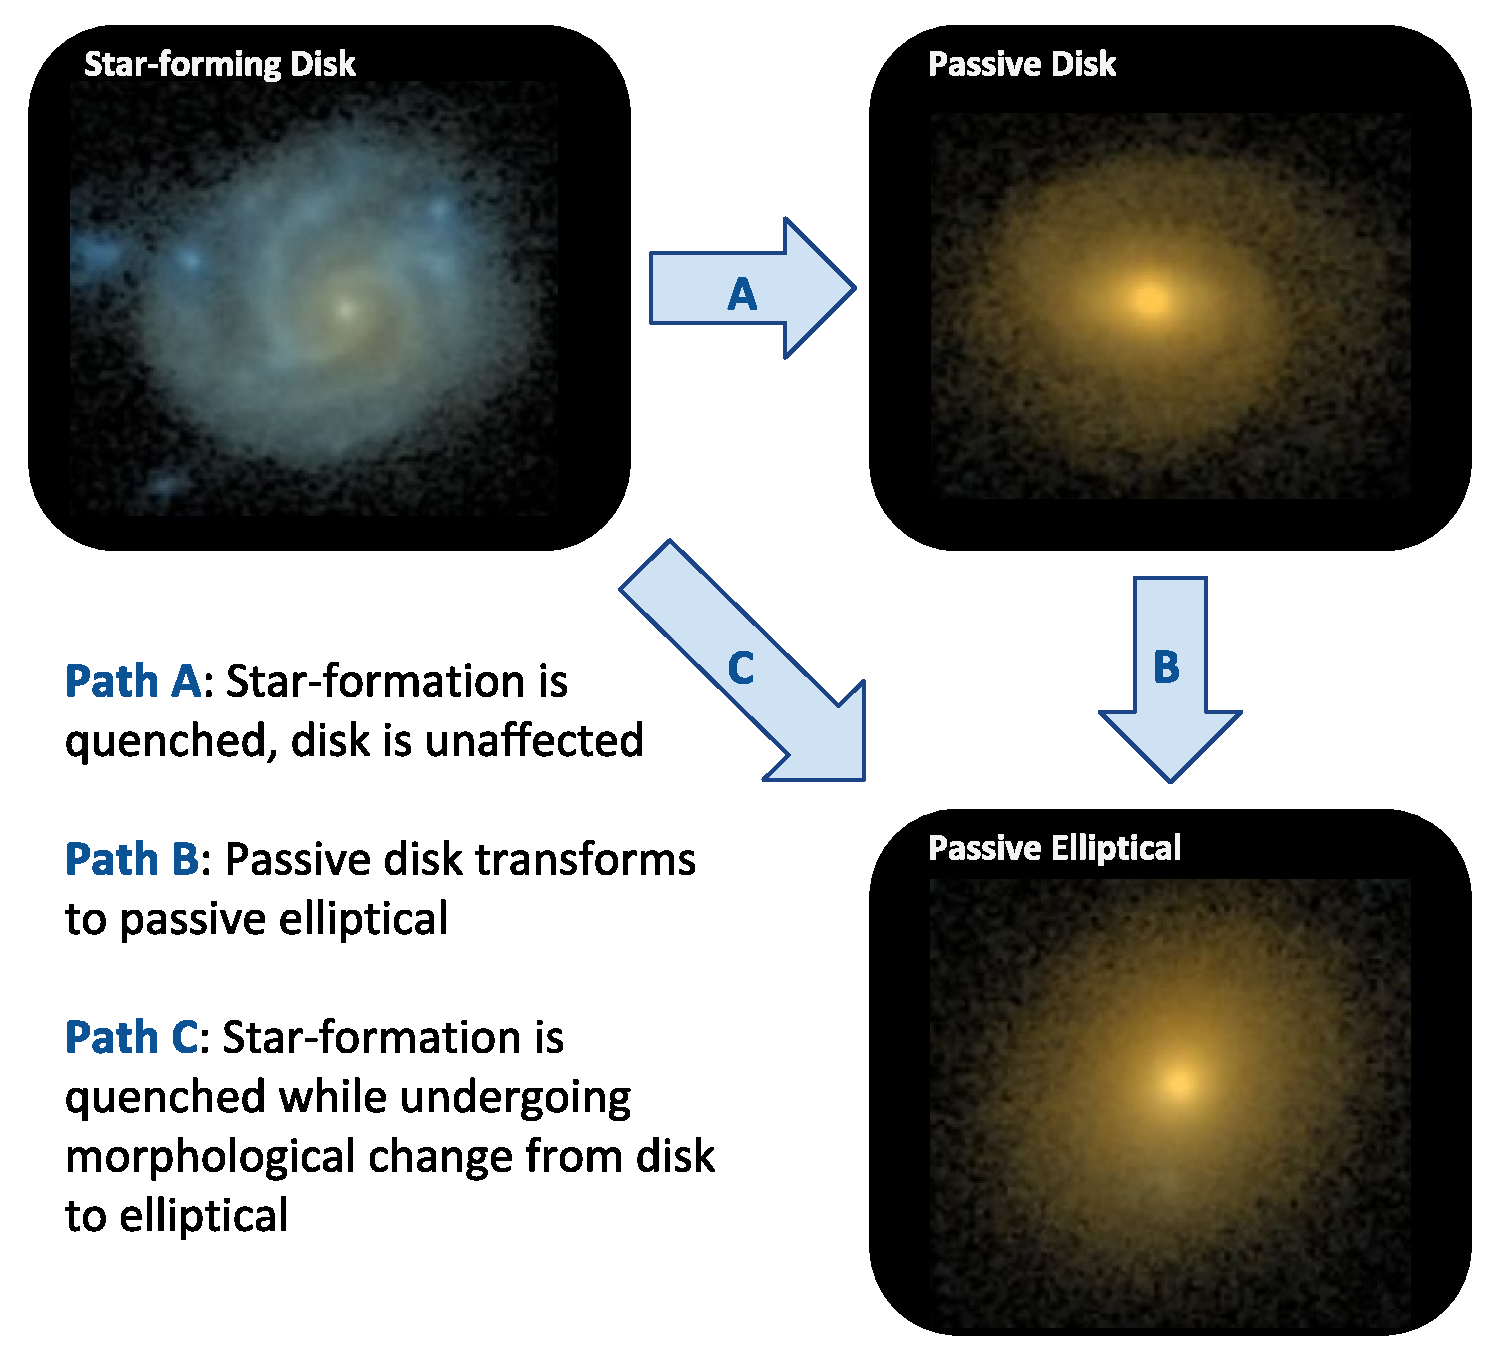
\includegraphics[width=3.5in]{figures/cartoon.pdf}
\caption{Cartoon representing three common evolutionary pathways of star-forming disc galaxies. Path A represents an active star-forming galaxy which quenches without destroying the disc, becoming a red disc. Path B represents a red disc morphologically transition to red elliptical. Path C represents a blue discs simultaneously quenching and morphologically transforming to become a red elliptical. }
\label{fig:cartoon}
\end{figure}

Figure~\ref{fig:cartoon} is a simple schematic of dominant quenching pathways for typical galaxies. Path A represents the creation of red discs via a quenching mechanism which does not transform the morphology of a blue star-forming disc. Path B represents a morphological transformation of a red disc to a red elliptical galaxy. Path C represents the quenching of blue discs via a mechanism which simulaneously invokes a morphological transformation. If all galaxies adhered to the standard color-morphology relationship, one could deduce that all galaxies follow this path. The existance of the red disc population asserts that Path A is also a viable channel. If these were the only two channels, we would expect pile ups of red discs at all masses as the Universe evolves. We observed such pile ups for low mass red disc galaxies (Figures~\ref{fig:all_plot} and \ref{fig:f_results}), but not for massive galaxies. This suggests that Path B, the depletion of red discs via a later morphological transformation, is necessary to deplete the pool and counteract the pile up effect, and has increasing significance in higher mass galaxies.  


\subsection{Red disc fraction ($f_{R|D})$ and red sequence disc fraction ($f_{D|R}$): limiting cases}
To help understand the influences of the different quenching mechanisms Paths A, B, and C (Figure~\ref{fig:cartoon}), we explore limiting cases of the relative rates of these pathways and their influence on the red disc and red sequence disc fractions. A summary of these effects are displayed in Table~\ref{tab:arrows}. As in the previous section, we only discuss increases/decreases in fractions with \emph{increasing} cosmic time; that is, from right to left in the plots shown in Figure~\ref{fig:f_results}.

\subsubsection{Limiting case 1: Path A only}

In this scenario, blue discs may quench and retain their disc structure, but no morphological transformation occurs for either type. This results a depletion in the the number of blue discs at an equivalent rate as the build-up of red discs. A decrease in blue discs and increase in red discs both result in increases in $f_{R|D}$, so we would observe only increasing values of $f_{R|D}$ in Figure~\ref{fig:f_results}. Similarly, an increase in red discs coupled with no change in red ellipticals would result in a pure increase of the fraction of discs on the red sequence, $f_{D|R}$.

The creation of red discs via Path A requires quenching mechanisms which do not significantly alter the disc's morphology. Possible mechanisms include mass-quenching or AGN-feedback, which both induce quenching by cutting of the galaxy's gas reservoir required for ongoing star-formation. Mass-quenching occurs when a galaxy halo grows to a critical mass that induces virial shocks which heat the gas \citep{Schawinski2007,Birnboim2003,Cattaneo2006}. Since this type occurs in high mass galaxies, this could explain the increasing abundance of red discs observed in the higher mass bins (Figure~\ref{fig:all_plot}). Dilution of gas in massive galaxies due to such shock-induced heating can cause it to become more vulnerable to AGN feedback \citep{Dekel2006}, whereby accretion onto the galaxy's supermassive black hole generates strong outflows of energetic material and hard, non-thermal radiation. These AGN-driven winds may then terminate star-formation by heating the gas or expelling it completely from the galaxy, causing a quench. Such a process is not likely to induce a morphological transformation, and therefore could be another valid mechanism for creating a quenched disc.

Red discs can also be the product of merger events. Simulations have shown cases of rotationally supported discs surviving or reforming after a major merger. This seems to be possible under conditions such that the progenitor discs are gas-dominated \citep{Governato2009,Springel2005a}; for \citet{Robertson2006} discs were only re-formed if the gas-fractions exceeded $f_{gas}>0.5$. Under these conditions, it would be more likely to form low-mass discs, given that gas fraction tends to anti-correlated with stellar mass \citep{Kannappan2004,Bell2000}. Perhaps this mechanism could explain some portion of the low-mass red disc population. However, regrown discs in these simulations tend to exhibit star-formation activity. If the merger-disc regrowth event enhances star-formation only briefly, then perhaps the remaining gas is used up on a shorter time-scale, leading to a low-mass red disc. \citet{Sparre2017} find that although most of the new discs were star-forming, some were immediately quenched in simulations which incorporated particularly strong AGN feedback. 



\subsubsection{Limiting case 2: Path B only}

Path B represents the depletion of red discs as they morphologically evolve to build up the population of red ellipticals. If blue discs are no longer quenching to build up the population of red discs, then we would only observe decreases in both $f_{R|D}$ and $f_{D|R}$ as the number of red discs decreases, blue discs remain constant, and red ellipticals increase. 

Our results suggests that Path B, the morphological transformation of red discs, is more common for high mass red discs than their low mass counterparts. It has been long suggested that major-mergers are the dominant mechanism for transforming the majority disc-like galaxies to an elliptical morphology \citep{Toomre1977,Schweizer1982,Schweizer1990}, with multiple minor-mergers being the second-most dominant~\citep{Bundy2009,Hopkins2010b}. Studies using observations of close pairs have shown the galaxy merger rate increases with mass, both in the local Universe \citep{Xu2004,Patton2008,Domingue2009,Robotham2014,Casteels2014} and out to $z\sim1$ \citep{Xu2012,Bundy2009}, which agrees with predictions from both empirical models and dynamical simulations \citep{Hopkins2010a,Hopkins2010b,Maller2006}. \citet{Casteels2014} find the merger rate is as much as three times higher for massive ($\rm log(M/M_{\odot})\sim11.25$) than for lower mass ($\rm log(M/M_{\odot})\sim8.25$) galaxies, using a similar mass range probed in our study. The increasing merger rate with mass may explain why massive red disc galaxies do not tend to stay in this phase long before merging, while low mass galaxies which become red discs are more persistant in that phase. 
 

\subsubsection{Limiting case 3: Path C only}
We now consider the scenario in which blue disc galaxies only quench via processes which simutaneously destroy their discs. The most extreme consequence of this scenario is of course a complete absence of red disc galaxies, which would give $f_{R|D}=f_{D|R}=0$ for all redshifts. Allowing for an initial population of red discs, we can explore how $f_{R|D}$ and $f_{D|R}$ would evolve if Path C were to suddeny become the only option. 

The evolution of $f_{R|D}$ is dependent on the growth/depletion of red and blue discs. In this scenario red discs are not building up, nor are they transforming morphologically; therefore their number remains constant, and the evolution of $f_{R|D}$ is solely dependent on the blue discs. If blue discs only evolve via path C, their number could only decrease, leading to an overall increase of $f_{R|D}$. 
$f_{D|R}$ in this scenario is only affected by the net change of red ellipticals, whose numbers are increasing via Path C. Therefore this scenario would give a decrease of $f_{D|R}$.% However, it is also possible for red ellipticals to merge and grow in mass, causing them to leave or enter a given mass bin. Thus a net increase or decrease in the number of ellipticals will depend on the relative rate of Path C and the merger rate at each mass. 

\subsubsection{Limiting case 4: No quenching pathways, only mass growth via star-formation}

Even in the limiting sceneario in which there are no quenching mechanisms or morphological transformations, the fractions in Figures~\ref{fig:all_plot} and~\ref{fig:f_results} would evolve due to star-formation in the blue discs. In a given mass bin, blue discs may enter from a lower mass bin or exit to enter a higher mass bin as they continuously increase their mass via star-formation. The net rate of blue galaxies entering/leaving a mass bin via star-formation can be estimated by the mass derivative of the mass function of blue galaxies times the specific star-formation rate $d\phi_{blue}/dm \times sSFR (m,t)$ \citep{Peng2010}. Using a Schechter (1976) mass function, $d\phi_{blue}/dm = (1+\alpha_s) - m/M^*$ with $\alpha_s = -1.4$ and $M^* = 10.28~(log(M/M_{\odot}))$ \citep{Ichikawa2017} and specific star-formation rate given by \citet{Peng2010} $sSFR(t) = 2.5(\frac{t}{3.5 Gyr})^{-2.2}Gyr^{-1}$, we find the net rate of change of blue discs \emph{due to star-formation only} is always positive for the masses and redshifts considered in Figure~\ref{fig:f_results}. 

Therefore, in the absence of quenching, we would observe a steady increase of the fraction of blue discs in Figure~\ref{fig:all_plot}. The flatness observed suggests that their numbers are depleting via Paths B or C at similar rates as their numbers are repleneshing each bin via star-formation. In $f_{R|D}$ we would only observe a decrease as the number of blue discs increased, and $f_{D|R}$ would remain constant as the number of blue discs do not enter the equation.

\begin{table}
\begin{tabular}{lcc}
\hline
\hline
net effect on:           & $f_{R|D}$      & $f_{D|R}$    \\
\hline
Path A only              &  $\uparrow$    &  $\uparrow$        \\
Path B only              &  $\downarrow$  &  $\downarrow$   \\
Path C only              &  $\uparrow$    &  $\downarrow$   \\
star-formation only      &  $\downarrow$  &  no effect   \\
\hline
\end{tabular}
\caption{Net effects on the red disc fraction $f_{R|D}$ and red sequence disc fraction $f_{D|R}$ for limiting single-scenario cases of transformative pathways A, B, C (Figure~\ref{fig:cartoon}) and mass growth via star-formation. $\uparrow$ represents an increase in repsective fractions with increasing cosmic time / decreasing redshift (right to left in Figure~\ref{fig:f_results}). This information can be used to find the dominant effects driving the trends in Figure~\ref{fig:f_results}. }
\label{tab:arrows}
\end{table}


\subsection{Identifying the dominant transformative pathways as a function of mass}
[This is the dryest of the dry sections and to be honest I'm not sure if this should be laid out all in words or if it's best summarizing all of this in another table]
In the context of the above discussion outlining the net effects of Paths A, B, C, and mass growth via star-formation, we will summarize the trends observed in Figure~\ref{fig:f_results} for each stellar mass bin and identify the most probable drivers of the trends. 

\subsubsection{$\rm 11.0<log(M/M_{\odot})<11.3$}
%purple stars

For galaxies in the highest mass bin, $f_{R|D}$ decreases from 0.36 to 0.28 since $z=1$. This suggests that the rate of occurance of Path B, the morphological transformation of red discs to elliptical, is strong with respect to paths A or C. Via Table~\ref{tab:arrows} it is possible that star-formation has an impact in this trend, however it is not expected to be the dominant driver given the flatness of the fraction of blue discs observed in Figure~\ref{fig:all_plot}.

$f_{D|R}$ decreases from 0.52 to 0.36, which could be driven by Path B or C. Given that a dominant Path C would cause an increase in $f_{R|D}$ (opposite of what we observe), it is more likely that Path B is the primary driver of this decrease. 

\subsubsection{$\rm 10.7<log(M/M_{\odot})<11.0$}
%Red squares

For galaxies in the second highest mass bin, $f_{R|D}$ is consistent with a slope of zero. This suggests that the rate of Path B is on par with the combined rates of A and C. As with the highest mass, star-formation is not expected to be a dominant contribution due to the flatness of the blue disc fraction in Figure~\ref{fig:all_plot}. 

$f_{D|R}$ is also consistent with a slope of zero. This suggests Path A is significantly strong to balance the decreasing effects of Paths B and C. 

\subsubsection{$\rm 10.4<log(M/M_{\odot})<10.7$}
%Blue Diamonds 

For galaxies in the second lowest mass bin, $f_{R|D}$ increases from 0.09 to 0.12. This indicates that paths A and C are dominating, meaning path B is less dominant as compared to the higher masses. 

$f_{D|R}$ increases from 0.29 to 0.37. This indicates that Path A dominates over both B and C.  

\subsubsection{$\rm 10.1<log(M/M_{\odot})<10.4$}
%Green triangles

$f_{R|D}$ increases from 0.03 to 0.14, indicating path B is not significant compared to A and C. 

$f_{D|R}$ is consistent with a slope of zero, indicating the rate of Path A is comparable to the combined effect of B and C. 

A summary of the above breakdown is as follows: Path B, the depletion of red discs via a morphological transformation to elliptical, operates at a higher frequency for more massive galaxies than the lower mass galaxies. In other words, lower mass galaxies are more likely to remain in a red disc phase, while high mass red discs are more likely to merge and transition to elliptical. Path A, the creation of red discs, is strongest for high masses, given by the trends of $f_{R|D},f_{D|R}$ and the larger abundance of red discs in the higher mass bins.  


\subsection{Looking forward: developing a model to reproduce observations}

Through observations of the evolution of the red disc population since $z=1$, we have deduced that massive galaxies are more likely to both enter a red disc phase and subsequently exit the stage via a morphological transformation, while low mass discs which enter a passive stage are more likely to remain in that phase than continue their evolution. To quantify and verify this interpretation would require further work, such as a semi-analytical model which could reproduce these observations given parameters describing the rate of occurrences of the different evolutionary pathways shown in Figure~\ref{fig:cartoon}. A complete model is beyond the scope of this work, but an example of a simple toy-model approach is given in Appendix A. Our simple model was not able to constrain values for all parameters implemented, but it did detect a mass-dependence on the rate at which blue discs transform to red discs, which agrees with our interpretations thus far. 


\section{Conclusions}
\label{sec:conclusions}

We have investigated the population of passive disc galaxies across a range of stellar masses and redshifts from z=1 to the present epoch. We used morphological classifications from Galaxy Zoo: Hubble and rest-frame colours from UltraVISTA. Using data from artificially-redshifted \ferengi2 images to quantify the known redshift bias in the GZ classifications, we derived expressions to correct the incompleteness in the number of discs and ellipticals detected as a function of redshift. The relative population statistics were described in terms of the fraction of disc galaxies that are red $f_{R|D}$ and the fraction of disc galaxies on the red sequence $f_{D|R}$. Our main conclusions are as follows:

\begin{itemize}

\item{$f_{R|D}$ and $f_{D|R}$ decrease from $z=1$ to $z=0.3$ for massive galaxies, and increase for the least massive galaxies.}

\item{Low mass galaxies which experience a passive disc phase are more likely than massive galaxies to remain discs, while massive galaxies are more likely to continue their evolution by transforming to passive ellipticals. Additional data are required to properly constrain semi-analytic models that might further elucidate the physical processes that generate the observed population trends.}


\end{itemize}





%%%%%%%%%%%%
%%% ACKNOWLEDGMENTS
%%%%%%%%%%%%
The data in this paper are the result of the efforts of the Galaxy~Zoo~Hubble volunteers, without whom none of this work would be possible. Their efforts are individually acknowledged at \url{authors.galaxyzoo.org}. Please contact the author(s) to request access to research materials discussed in this paper. 


MG, CS, MB, and LF gratefully acknowledge support from the US National
Science Foundation Grant AST1413610.

This publication makes use of data products from the Two Micron All Sky Survey, which is a joint project of the University of Massachusetts and the Infrared Processing and Analysis Center/California Institute of Technology, funded by the National Aeronautics and Space Administration and the National Science Foundation.

This project made heavy use of the Astropy packages in Python \citep{Robitaille2013}, the \texttt{seaborn} plotting package \citep{Waskom}, and the Tool for OPerations on Catalogues And Tables (TOPCAT), which can be found at \url{www.starlink.ac.uk/topcat/} \citep{Taylor2005}. 

Funding for the SDSS and SDSS-II has been provided by the Alfred P. Sloan
Foundation, the Participating Institutions, the National Science Foundation,
the U.S. Department of Energy, the National Aeronautics and Space
Administration, the Japanese Monbukagakusho, the Max Planck Society, and the
Higher Education Funding Council for England. The SDSS website is
\url{http://www.sdss.org/}. 

The SDSS is managed by the Astrophysical Research Consortium for the
Participating Institutions. The Participating Institutions are the American
Museum of Natural History, Astrophysical Institute Potsdam, University of
Basel, University of Cambridge, Case Western Reserve University, University of
Chicago, Drexel University, Fermilab, the Institute for Advanced Study, the
Japan Participation Group, Johns Hopkins University, the Joint Institute for
Nuclear Astrophysics, the Kavli Institute for Particle Astrophysics and
Cosmology, the Korean Scientist Group, the Chinese Academy of Sciences
(LAMOST), Los Alamos National Laboratory, the Max-Planck-Institute for
Astronomy (MPIA), the Max-Planck-Institute for Astrophysics (MPA), New Mexico
State University, Ohio State University, University of Pittsburgh, University
of Portsmouth, Princeton University, the United States Naval Observatory and
the University of Washington. 

\bibliographystyle{mn2e}
\bibliography{/home/mel/Documents/Papers/library}  


\newpage
\clearpage

\appendix

\section{Toy-model approach to constrain rates of different evolutionary pathways}

Our observations of the fractional evolution of different morphological and activity types of galaxies since $z=1$ are well-suited for the implementation of a model to constrain the frequencies of different evolutionary pathways. Here we present our preliminary attempt at a toy model used to reproduce our observations, given different sets of input parameters. This is intended to be a suggested starting point for the further development of a sophisticated, semi-analytic model to describe and constrain potential rates of quenching and morphological evolution. 

We implement a simple toy model to track the change in $f_{R|D}$ and $f_{D|R}$, given a range of parameters representing the quenching and morphological transformation rates for galaxies at fixed stellar mass. We begin by considering the rate of change in the number of blue discs ($dN_{BD}/dt$), red discs ($dN_{RD}/dt$), and red ellipticals ($dN_{RE}/dt$). In a given mass bin, the change in numbers for each population will depend on several parameters, illustrated visually in Figure~\ref{fig:cartoon}.

\subsubsection{Blue Disks}
First, galaxies in a blue bin may transition into a red disc bin via a quenching process that does not destroy its disc; we define this rate as $r_{BD \rightarrow RD}$, representing the fraction of blue galaxies to transition to red discs per Gyr (path A in Figure~\ref{fig:cartoon}). Blue galaxies may also exit a bin via a quenching process which \emph{does} destroy the disc; this fraction per Gyr we define as $r_{BD \rightarrow RE}$ (path C in Figure~\ref{fig:cartoon}).

The number of galaxies in a blue disc bin will also change due to star formation, which brings active galaxies from a lower mass bin into the current mass bin. To account for this term we use the formalism outlined by \citet{Peng2010}, in which this rate of change is given by $(\alpha + \beta)sSFR$. Here $\alpha = d\phi_{blue}/dm$ is the derivative of the mass function for blue galaxies, which equates to $\alpha = (1+\alpha_s) - m/M^*$ for a mass function described by the Schechter (1976) function. We use best-fit parameters for blue galaxies measured by \citet{Ichikawa2017}, which give $\alpha_s = -1.4$ and $M^* = 10.28 ~(log(M/M_{\odot}))$. Following the method of \citet{Peng2010}, we let $\beta=0$, both for simplicity, and because their conclusions found not to be strongly dependent on $\beta$. Last, the specific star-formation rate is given by $sSFR(t) = 2.5(\frac{t}{3.5 Gyr})^{-2.2}Gyr^{-1}$ \citep{Peng2010}.

Accounting for all sources and sinks of blue discs entering or exiting a bin of given mass, the rate of change of blue discs can be written fully as:

\begin{equation}
\frac{dN_{BD}}{dt}\Big\rvert_{m} = \Big(-r_{BD \rightarrow RD} - r_{BD\rightarrow RE} -\alpha(m) sSFR(t) \Big)N_{BD}
\label{eqn:BD}
\end{equation}

\subsubsection{Red Disks}
Galaxies exiting a blue bin as they quenched without disrupting their discs enter the pool of red discs, increasing $N_{RD}$ for a given mass bin. Red discs also may undergo a morphological transformation, depleting the pool of red discs as they enter the red elliptical bin (path B in Figure~\ref{fig:cartoon}). The fraction of galaxies to undergo this pathway per Gyr is denoted as $r_{RD->RE}$. Combining these factors gives the expression: 

\begin{equation}
\frac{dN_{RD}}{dt}\Big\rvert_{m} = + r_{BD \rightarrow RD}N_{BD} - r_{RD \rightarrow RE}N_{RD}
\label{eqn:RD}
\end{equation}

\subsubsection{Red Ellipticals}
In this simple model, it is assumed that red, passive ellipticals are the final state in a typical galaxy's evolution. Therefore $N_{RE}$ will always be increasing from the transformation from blue discs and red discs to red ellipticals ($r_{BD \rightarrow RE}$, $r_{RD \rightarrow RE}$). However, the number of red ellipticals \emph{in a single mass bin} may still decrease due to ellipticals at the given mass merging to enter a bin of red ellipticals at a higher mass. Similarly, their number can increase as ellipticals from a lower mass bin merge to enter the current mass bin. A complete, semi-analytic model would consider this full range of possibilities and couple the resulting equations appropriately amongst all mass bins. For the purposes of this simple model, we opted to represent the total, net rate of change of the number of red ellipticals as a single parameter, $\kappa_{RE}$, which we note may be positive or negative, depending on whether more ellipticals are entering or leaving the given mass bin. 

\begin{equation}
\frac{dN_{RE}}{dt}\Big\rvert_{m} = \kappa_{RE} N_{RE}  
\label{eqn:RE}
\end{equation}

We exclude the contribution from blue ellipticals from the model for maximum simplicity, and because they represent only a small fraction of the total population at most masses. A complete version of the model would include this population. We initialize our model using the observed relative numbers of blue discs, red discs, and red ellipticals measured at $z=1$, then use the model to compute their evolution to $z=0.3$ using a range of values for each of the four parameters in four mass bins. For $r_{BD \rightarrow RD}, r_{BD \rightarrow RE},$ and $r_{RD \rightarrow RE}$, we test 25 values between 0 and 1, and 25 values between -1 and 1 for $\kappa_{RE}$. We note that a complete model would explore time-varying rates, but for the purposes of simplicity in our toy-model we only experiment with static parameters. For each mass bin, the model was implemented for each permutation of the four rate parameters. The success of each run was evaluated using a $\chi^2$ metric; these results are shown for each mass bin in the corner-plot in Figure~\ref{fig:corner}. The bins are weighted by $1/\chi^2$, such that white regions represent the rate parameters that yield the lowest $\chi^2$, and black representing the largest.

\begin{figure*}
\centering
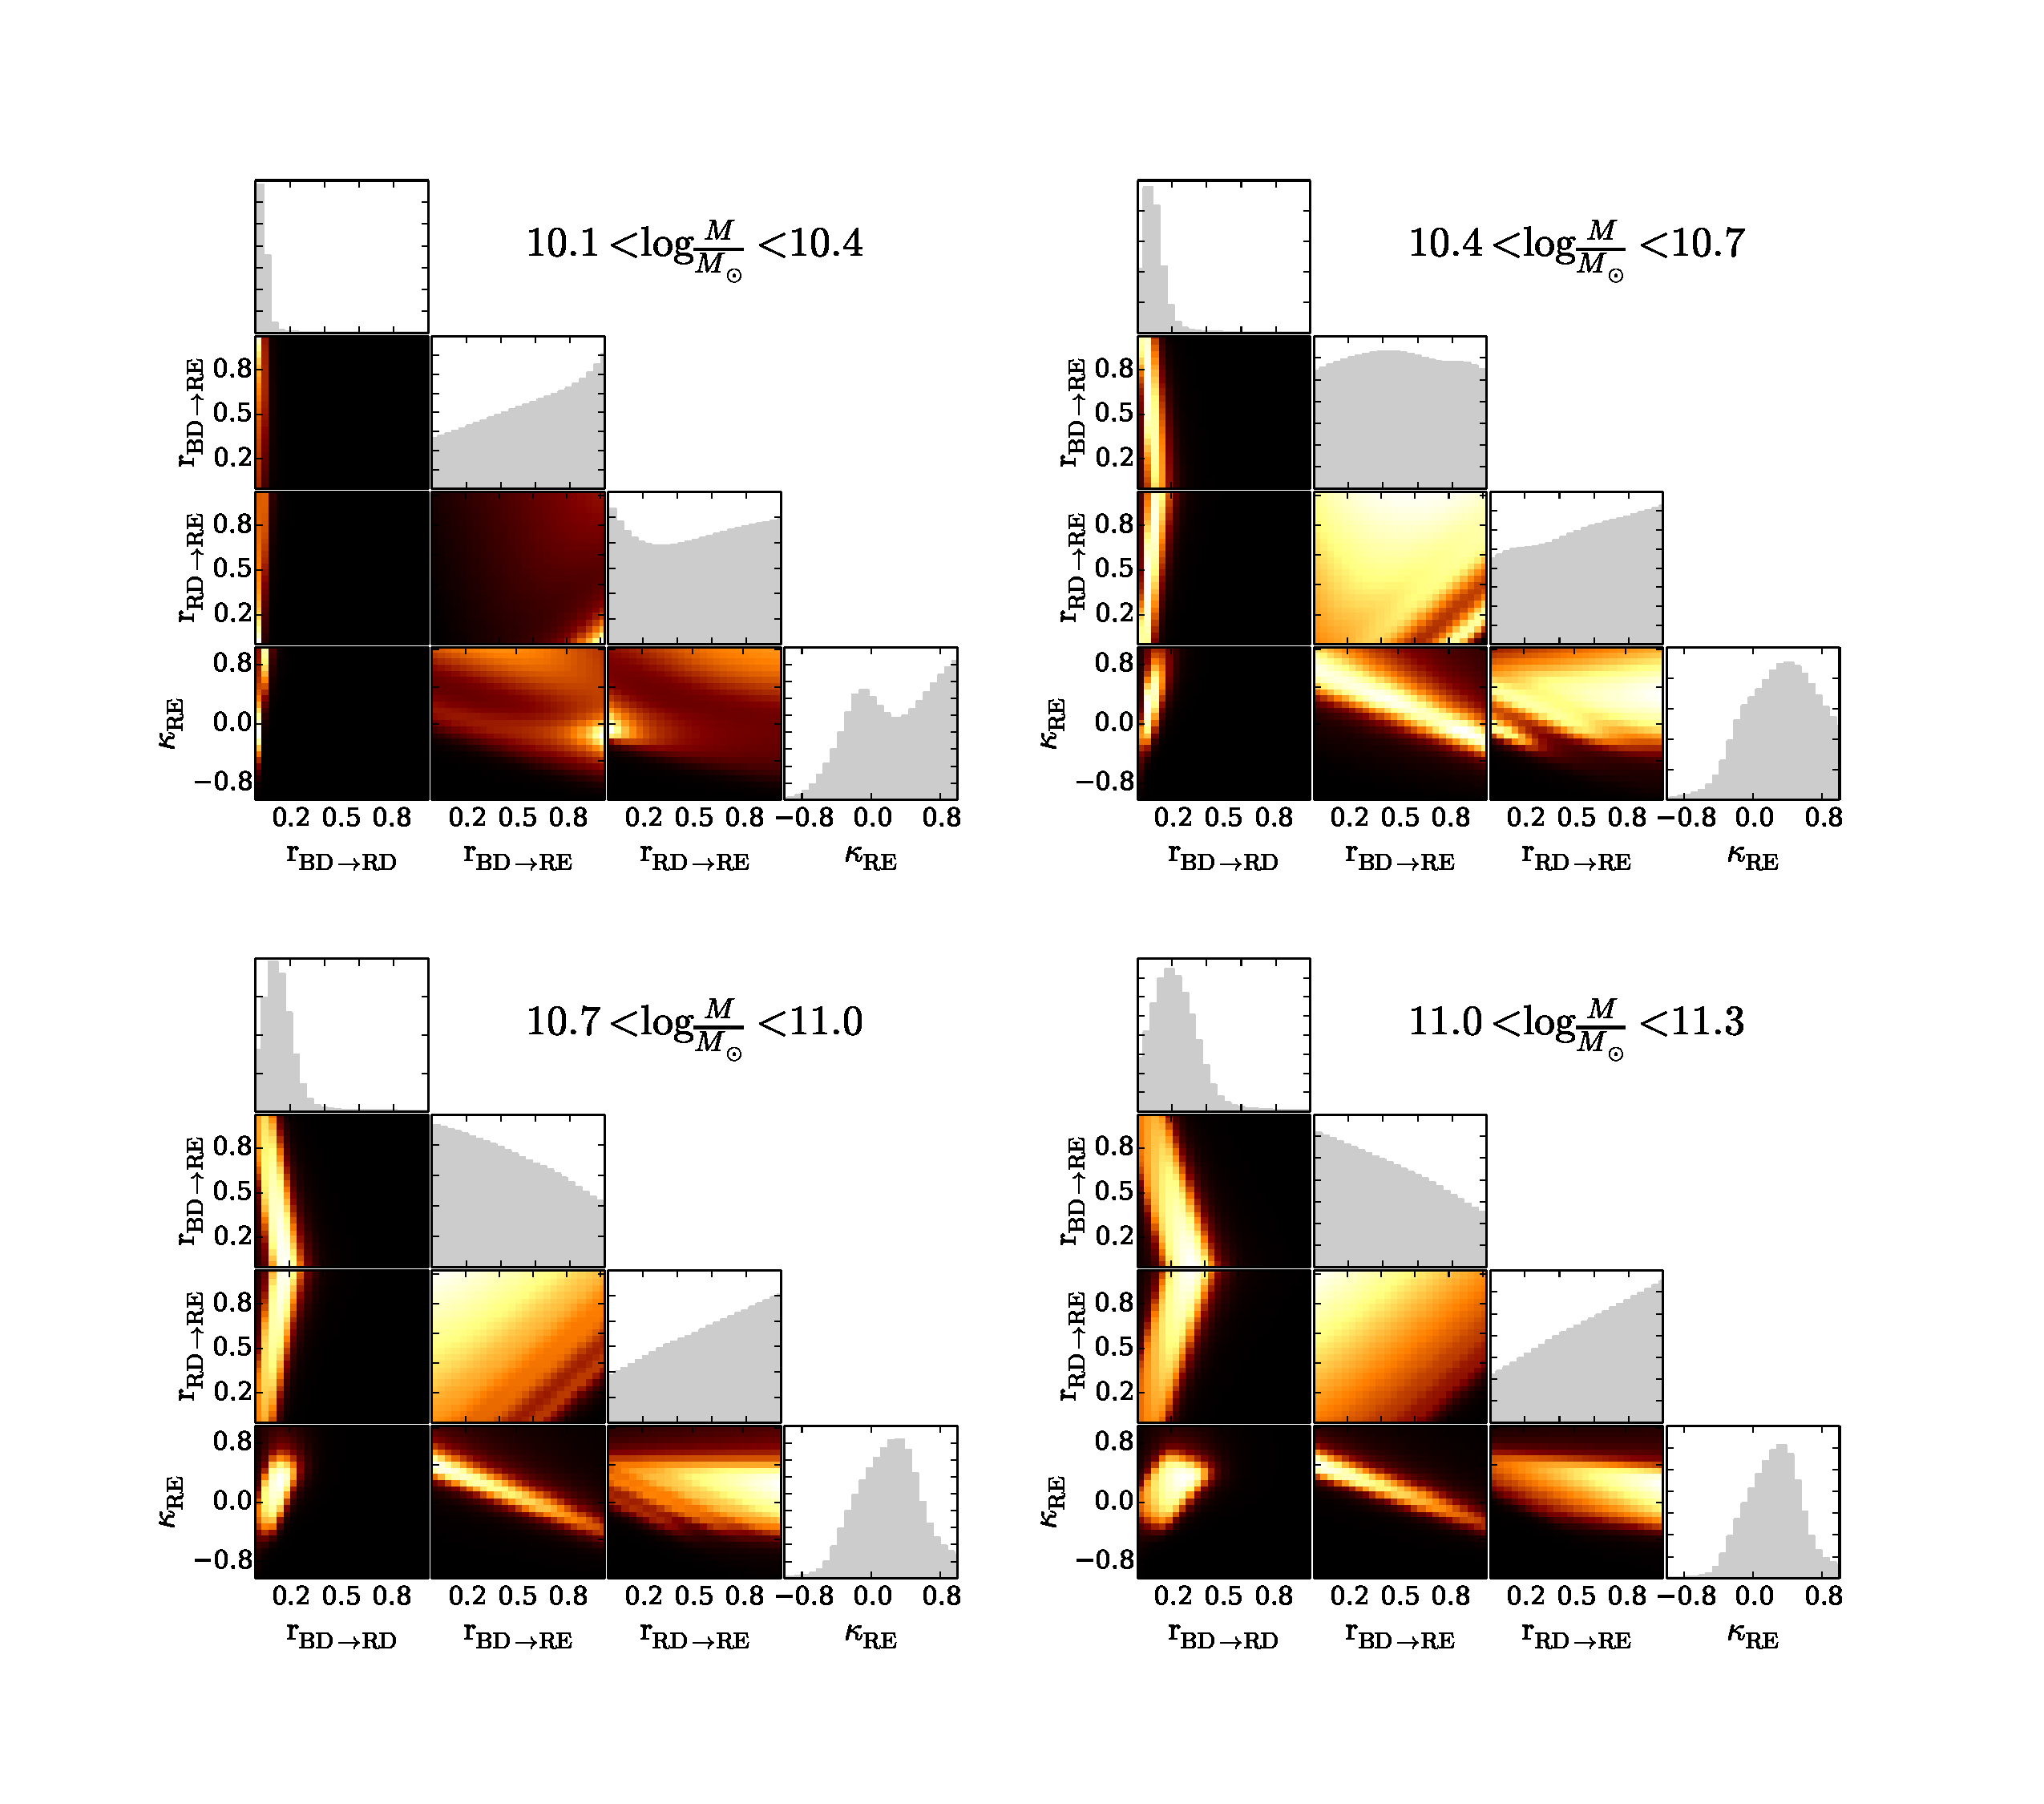
\includegraphics[width=\textwidth,trim={0cm 0cm 2cm 1cm},clip]{figures/corner_plot.pdf}
\caption{Results of the grid-search for the best-fit rate parameters $r_{BD \rightarrow RD}, r_{BD \rightarrow RE}, r_{RD \rightarrow RE}$, and $\kappa_{RE}$ for four mass bins. The units for all rate parameters is $\rm Gyr^{-1}$. 25 equally-spaced values were tested between (0,1) for each parameter, with the exception of $\kappa_{RE}$ which was tested for 25 values between (-1,1); these are represented by the 25 bins on each axis. Each bin is weighted by $1/\chi^2$, such that white regions correspond to parameters which produced the lowest $\chi^2$, and black representing the highest. There is a strong result in the dependence of $r_{BD \rightarrow RD}$ with mass, such that the fraction of blue discs which transition to red discs (ie, quench without disrupting the disc), increases for more massive galaxies. The other parameters are less constrained by this model; therefore a more complex semi-analytic model will be necessary for obtaining the precise values of these rates, and is the subject of future work.}
\label{fig:corner}
\end{figure*} 

We find a strong mass dependence on the fraction of blue galaxies to quench to red discs ($r_{BD \rightarrow RD}$), or Path A in Figure~\ref{fig:cartoon}. Our observations of $f_{R|D}$ and $f_{D|R}$ are most closely reproduced when $r_{BD \rightarrow RD}$ = [0.05, 0.07, 0.1, 0.2] $\rm Gyr^{-1}$ for masses $\rm log(M/M_{\odot})$ = [10.25,10.55,10.85,11.0] These values for $r_{BD \rightarrow RD}$ correspond to the peaks of the 1-D histograms shown in Figure~\ref{fig:corner}. This increase of $r_{BD \rightarrow RD}$ with mass could suggest either: 1) more massive galaxies are more likely to undergo quenching processes which do not destroy their discs, or 2) less massive galaxies simply quench less frequently overall, via any pathway. 


 Analysis of the next parameter in the low mass bin, $r_{BD\rightarrow RE}$, suggests that the former is more likely, given the peak of $r_{BD \rightarrow RE}$ at $>0.9 ~\rm Gyr^{-1}$. The high rate of low-mass blue discs quenching to red ellipticals is evidence that they do not quench any less frequently than high mass galaxies, and the increase of $r_{BD \rightarrow RD}$ with mass is indeed consistent with quenching processes less likely to destroy the disc of massive galaxies. However, this result is not nearly as constrained, given the broad distribution of likelihoods for this parameter. $r_{BD \rightarrow RE}$ is even less constrained for all higher masses. The degeneracies evident in this rate and $r_{RD \rightarrow RE}$ make it clear that our model is not sufficient to constrain the relative frequencies of the processes involved in quenching and morphological transformations; a more sophisticated model with the adjustments we have described thus far would be necessary to paint the full picture. 




\end{document}
